\section{System Implementation}
This section will discuss about the system implementation by firstly focusing on the backend part of the mobile application, moving then to consider also parameters editing, so the web application part that allows to do that.
% Flutter state management spostato più in alto essendo backend posso dire
\subsection{Firebase}
\subsubsection{Firebase Authentication}
\label{subsubsec:firebaseAuthentication}
Setting up the Authentication was pretty straightforward, as also previously explained (see \cref{subsubsec:authenticationService}). All it took was going to the firebase console in the project settings and register both the mobile application and the web one. After that, in the authentication tab the desired Sign-in providers have been enabled (in our case email/password and Google). The firebase platform and the underlying google structure handled the rest by generating both the API keys to access the firebase services and the OAuth 2.0 clients to authenticate the users.

% \begin{figure*}
%     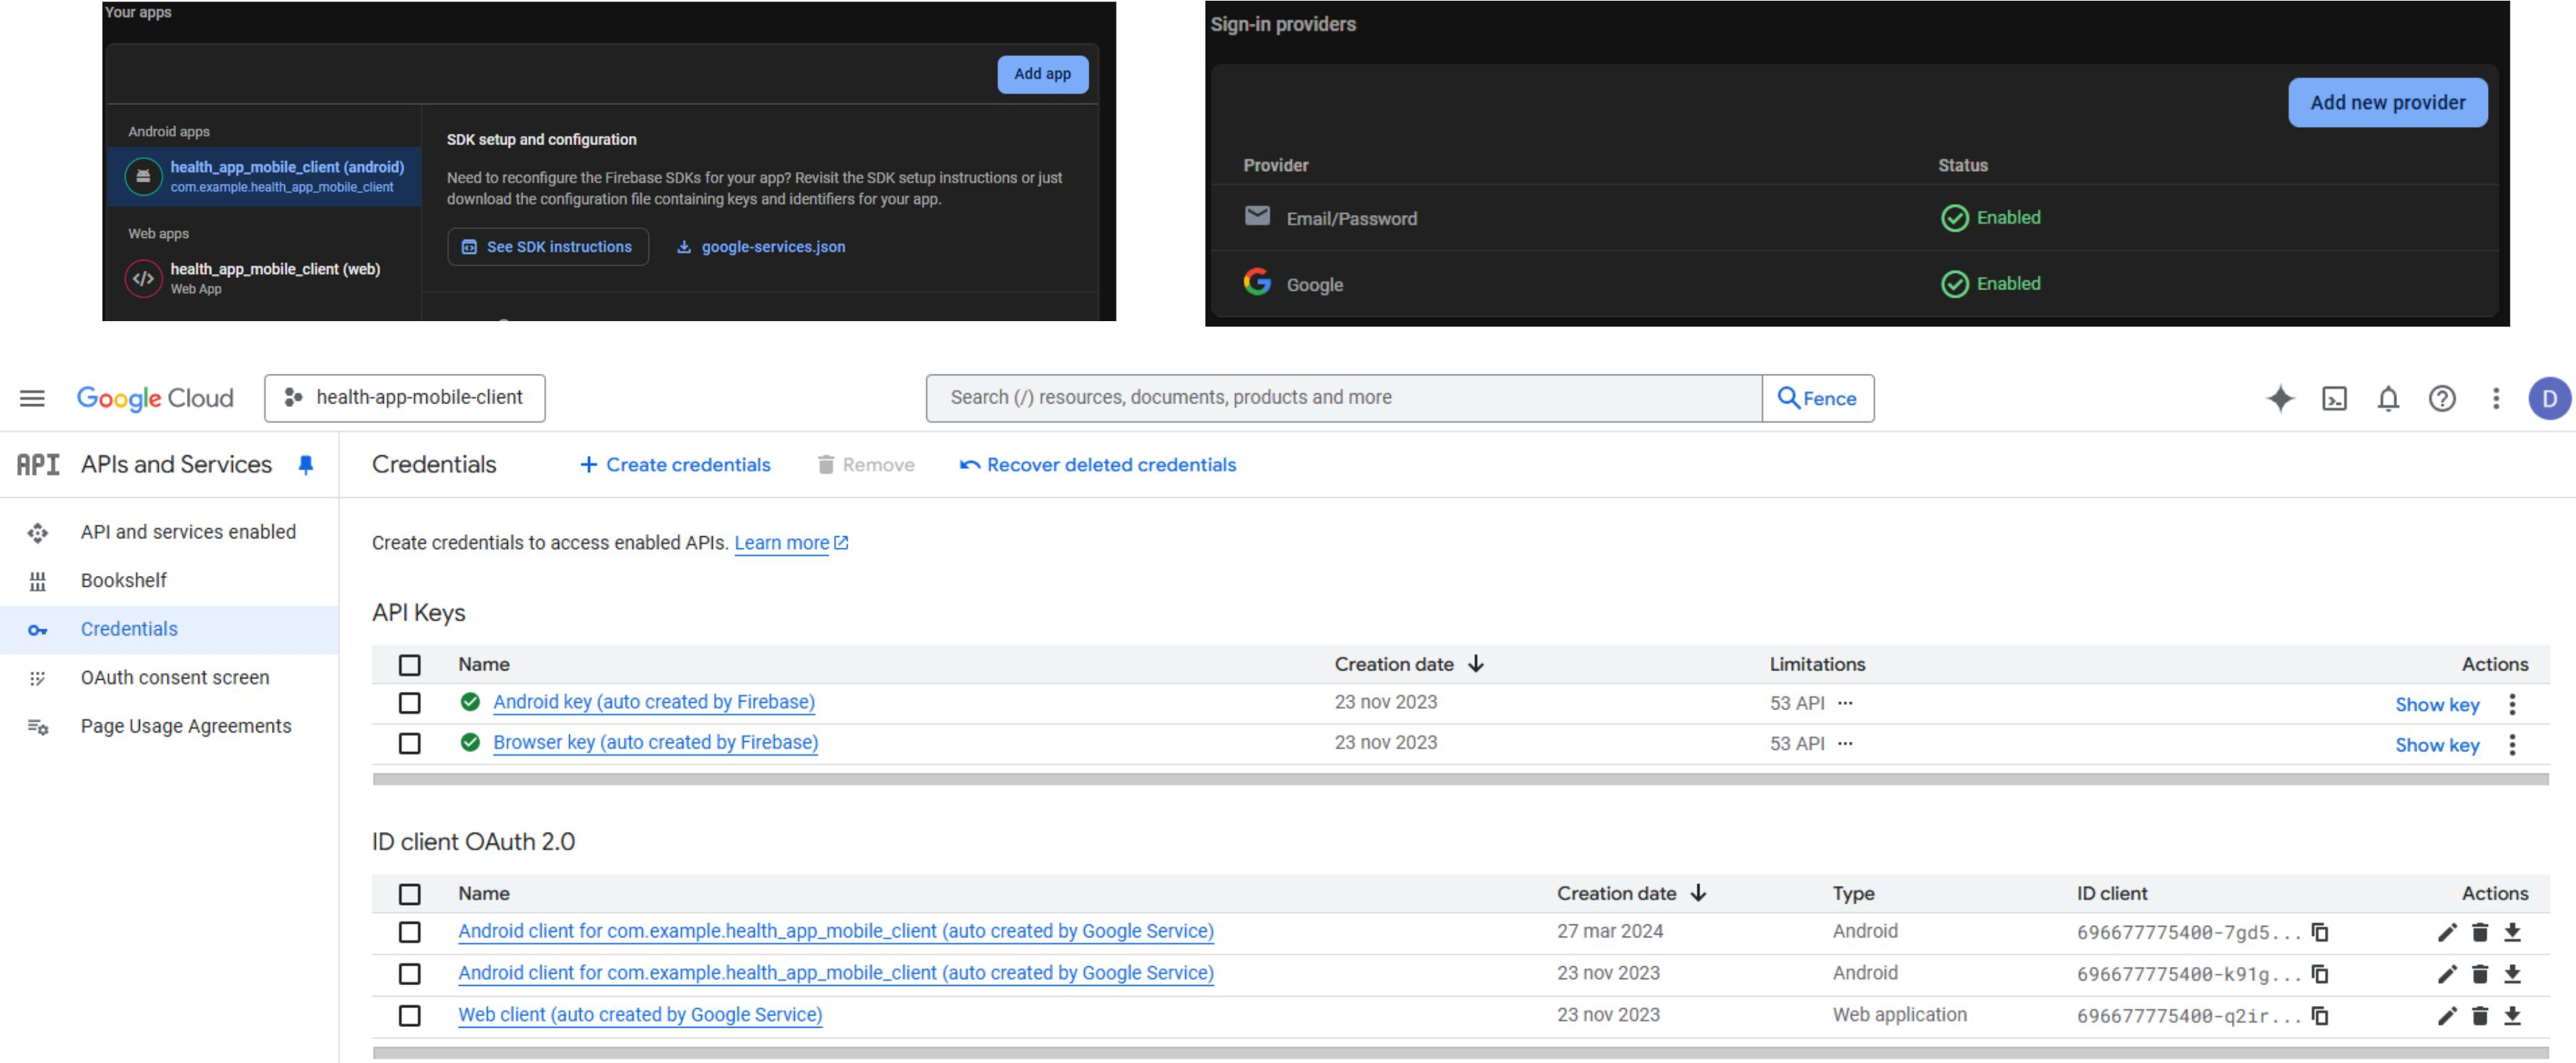
\includegraphics[width=1.0\linewidth]{./images/authentication.jpg}
%     \caption{Registered apps and sign-in providers in the firebase console and generated api keys and OAuth 2.0 clients in the cloud console.}
% \end{figure*}

\noindent In case of the email/password authentication approach, also email templates have been employed:
\begin{itemize}[nosep] % 'nosep' removes extra spacing between items
    \item \textbf{Email address verification:} once a user signs up, a confirmation email is sent to verify his registered email address.
    \item \textbf{Password reset:} in case a user forgets his password, he can request a password reset email.
    \item \textbf{Email address change:} in case a user change his email address, a confirmation email is sent to the original address, so that the user can review the change.
\end{itemize}
\newpage
\noindent At this point for the \textbf{mobile client} side the firebase dependencies (in particular firebase\_ui\_auth and firebase\_ui\_oauth\_google) have been employed to perform the authentication and the sign-in process. The already well made components already provide the possibility to sign-in or eventually register in case the user is not already registered, as well as manage the user profile once logged in. They are also highly customizable, allowing us to change the UI to match the app's theme. As additional logic, only the authentication state had to be handled in order to redirect the user to the home page once the authentication is successful. This has been done through a \texttt{StreamBuilder} widget and by using \texttt{FirebaseAuth.instance.authStateChanges()}, that notifies about the user's sign-in state as the source stream. In this way, any change is listened and if the user signs in or out the interface is updated coherently.

\noindent About the \textbf{web application client} instead, no already-made components were available, so the profile management screen like the mobile one has not been implemented, since it is an admin interface. The react \texttt{createContext} and \texttt{useContext} hooks have been employed to handle the authentication state: it was done by using a context in the react application and providing it at the root level so that the whole application could access the authentication state. This state is updated after performing authentication operations and the components that depend on it are updated accordingly, allowing to display the correct screens once authentication is performed.   

\begin{figure*}
    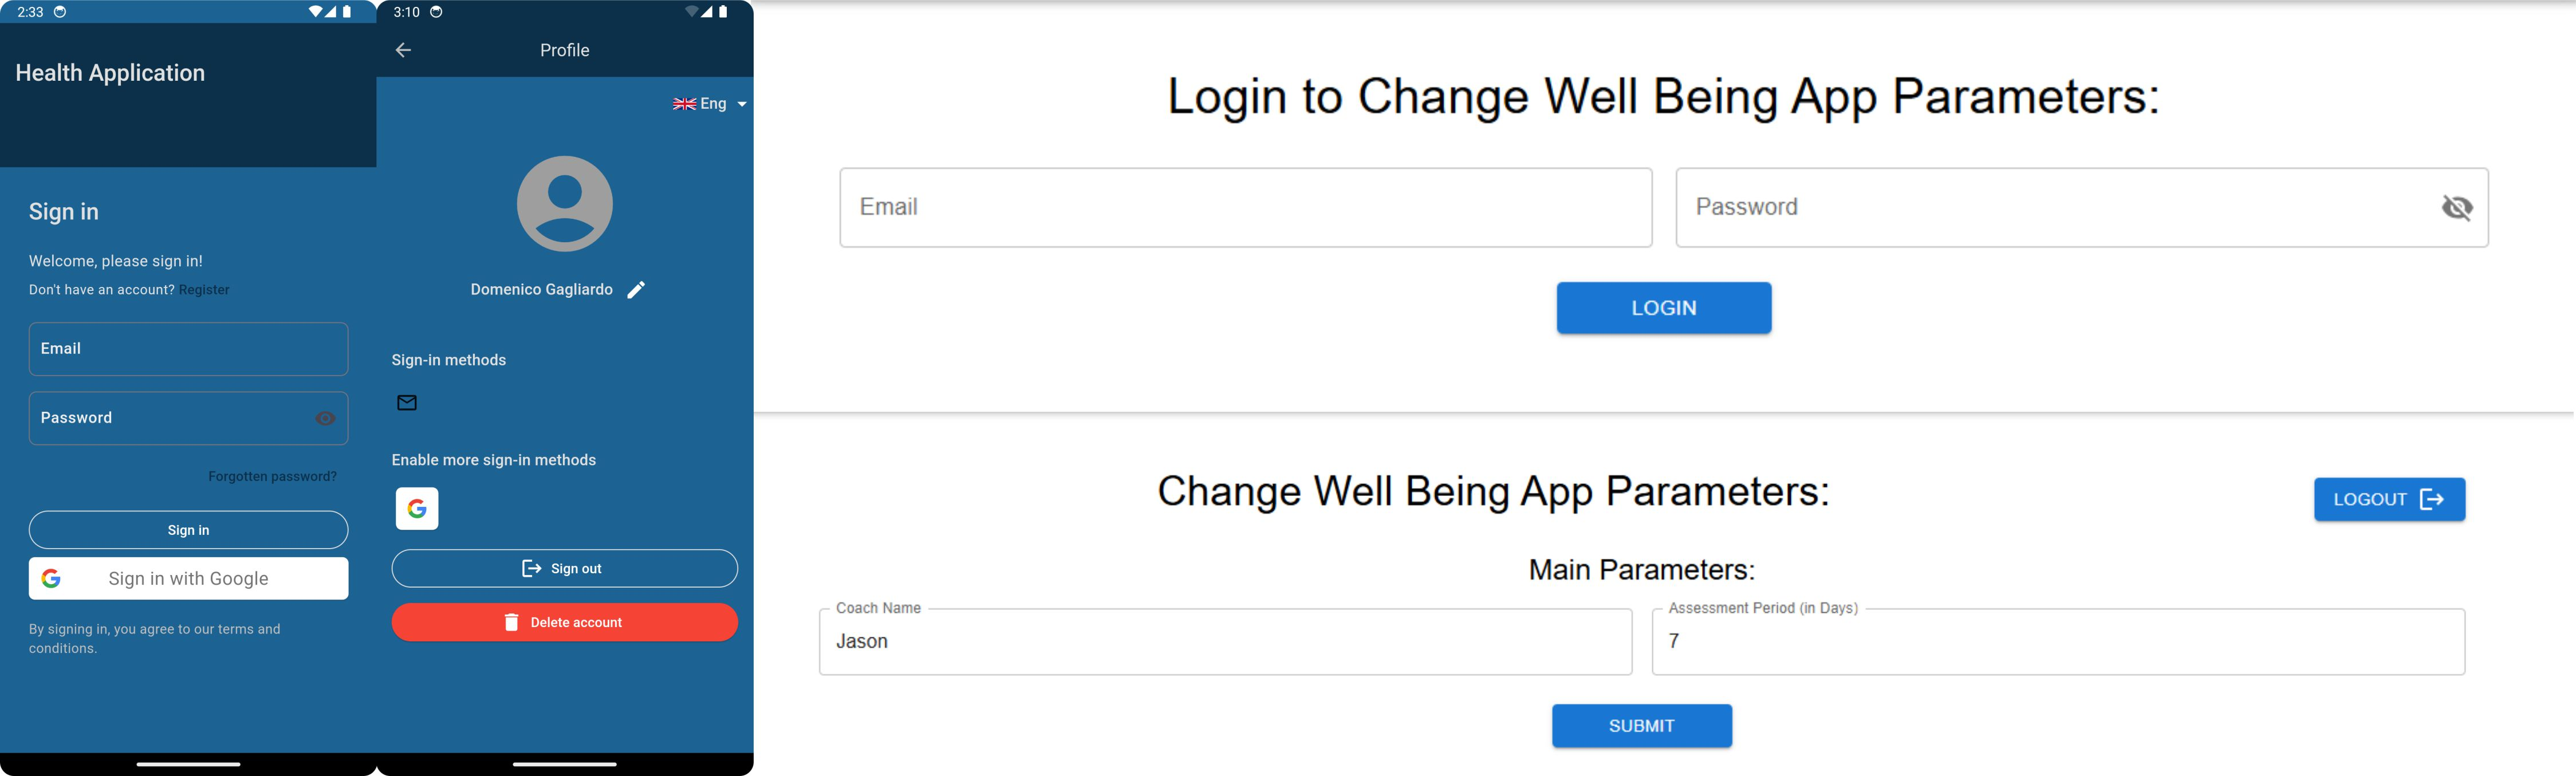
\includegraphics[width=1.0\linewidth]{./images/authenticationScreens.jpg}
    \caption{Authentication Screens of the mobile client (sign in and profile management) on the left and web client on the right.}
    \label{fig:authenticationScreens}
\end{figure*}
\newpage
\subsubsection{Cloud Firestore Database}
\label{subsubsec:cloudFirestoreDatabase}
Taking into account the data-related requirements (see \cref{tab:fr4}), the database has been implemented accordingly by storing all the data in the most efficient way possible. \newline The database structure is as follows:

\begin{itemize}[nosep] % 'nosep' removes extra spacing between items
    \item The \textbf{users} collection, used to manage main users informations, with each document having the following fields:
    \label{subsubsec:usersCollection}
    \begin{itemize}[nosep]
        \item The \texttt{UID} field, that uniquely identifies the user.
        \item The \texttt{goals} field (composed of \texttt{calories}, \texttt{sleep} and \texttt{steps} as inner fields) that represents the user's goals.
        \item The \texttt{language} field, that represents the app language set and preferred by the user.
        % wearable non in metrics ma scrivo così che fà cacare senò
        \item The \texttt{metrics} field (composed of \texttt{birthDate, height, nickname, sex, waist circumference, weight} and \texttt{wearable} as inner fields) that represents the user's personal information.
    \end{itemize}
\end{itemize}

\begin{itemize}[nosep] % 'nosep' removes extra spacing between items
    \item The \textbf{user\_data} collection, used to manage additional users informations, with each document having the following fields:
    \begin{itemize}[nosep]
        \item The \texttt{userId} field, that links those data with the corresponding user.
        \item The \texttt{current\_notification} field that used in combination with the \newline \texttt{notification\_counter} field allows to implement the notification logic (see \cref{subsec:notifications} for more details).
        \item The \texttt{lastBackupDate} field, that saves the last time that the user performed a backup of his data.
        \item The \texttt{weightData} array field that stores the user's weight information, implementing an history of this metric, alsop present in the \texttt{users} collection for each user. Each element of the array has the \texttt{date} and \texttt{weight} fields.    
        \item The \texttt{waistCircumferenceData} array field that stores the user's waist circumference information, implementing an history of this metric, alsop present in the \texttt{users} collection for each user. Each element of the array has the \texttt{date} and \texttt{waist} \newline \texttt{circumference} fields.
        % qui anche userId ma inutile perchè già in user_data non lo scrivo
        \item The \texttt{emotionalData} array field that stores the user's emotional information. Each element of the array has the \texttt{date}, \texttt{negative} and \texttt{positive} fields.
        \item The \texttt{bodyTestBalanceData} array field that stores the user's body balance information. Each element of the array has the \texttt{date}, \texttt{leftLeg}, \texttt{rightLeg} and \texttt{tandemWalk} fields.
        \item The \texttt{bodyTestStrengthData} array field that stores the user's body strength information. Each element of the array has the \texttt{date}, \texttt{absCount}, \texttt{gripTest}, \texttt{pushUpCount} and \texttt{squatCount} fields.
        \label{subsubsec:completedPills}
        \item The \texttt{completedLessons} array field that stores the user's completed lessons information. Each element of the array has the \texttt{lessonId} to which it refers to and a \texttt{completedPills} boolean array field used to store how many pills of the lesson have been read (true) or not (false).
        \item The \texttt{completedQuizzes} array field that stores the user's completed quizzes information. Each element of the array is the \texttt{quizId}: if present means that user has completed that quiz.
    \end{itemize}
\end{itemize}

\begin{itemize}[nosep] % 'nosep' removes extra spacing between items
    \item The \textbf{foodRecords} collection, used to manage the food informations for the users, with each document having the following fields:
    \begin{itemize}[nosep]
        \item The \texttt{userID} field, that links those data with the corresponding user.
        \item The \texttt{date} field, storing the food entry recording date.
        \item The \texttt{foodGroup} field, that identifies the type of food (like water, vegetables and so on).
        \item The \texttt{amount} field, that represents the food quantity (e.g. 250 ml if a liquid food or 250 gr if a solid food).
    \end{itemize}
\end{itemize}

\begin{itemize}[nosep] % 'nosep' removes extra spacing between items
    \item The \textbf{lessons} collection, used to manage the available lessons for the users, with each document having the following fields:
    \begin{itemize}[nosep]
        \item The \texttt{id} field, that uniquely identifies the lesson.
        \item The \texttt{quizId} field, that links the quiz related to that lesson.
        \item The \texttt{title} field, that represents the lesson title.
        \item The \texttt{titleIta} field, that represents the italian lesson title.
        \item The \texttt{pills} array field, that represents the list of pills that the lesson is made up of, where each element is a single pill.
        \item The \texttt{pillsIta} array field, that essentially is the italian version of the above \texttt{pills} field.
    \end{itemize}
\end{itemize}
\newpage
\begin{itemize}[nosep] % 'nosep' removes extra spacing between items
    \item The \textbf{quizzes} collection, used to manage the available quizzes for the users, with each document having the following fields:
    \begin{itemize}[nosep]
        \item The \texttt{id} field, that uniquely identifies the quiz.
        \item The \texttt{questions} array field, that represents the questions of that quiz. Each questions has the \texttt{questionText}, \texttt{correctAnswer} fields and \texttt{possibleAnswers} array field, that respectively represents the question, the correct answer and the list of possible answers, where each element is an answer.
        \item The \texttt{questionsIta} array field, that essentially is the italian version of the above \texttt{questions} field.
    \end{itemize}
\end{itemize}

\begin{itemize}[nosep] % 'nosep' removes extra spacing between items
    \item The \textbf{notifications\_text} collection, used to manage the mobile application parameters displayed for the users and editable by the admin through the web application. It is composed of 3 documents:
    \begin{itemize}[nosep]
        \item The first document, that contains two fields called \texttt{coach\_name} and \newline \texttt{assessment\_period} that represents the name of the app assistant and the length of the assessment perios (in days) used for the notification cycle (see \cref{subsec:notifications} for more details).
        \item The second document, that contains several strings fields used to customize the onBoarding experience of the user as well as the data insertion operations. We have up to three fields for the onBoarding (\texttt{onBoarding1,onBoarding2,onBoarding3}), 7 fields for the body test balance data insertion (\texttt{body\_test\_balance1} up to 7), 6 fields for the body test strength data insertion (\texttt{body\_test\_strength1} up to 6), one field for the emotional data insertion (\texttt{emotional\_life\_test}), one field for the assessment (\texttt{assessment}) and one field for the food insertion (\texttt{daily\_reminder\_food}).
        \item The third document, that similarly to what has been done with the lessons and quizzes, contains the italian version of the second document.
    \end{itemize}
\end{itemize}
\newpage
\subsection{User OnBoarding and Registration}
As explained before (see \cref{subsubsec:firebaseAuthentication}), the user registration and sign-in process is mainly managed by the firebase authentication service. However, some additional initialization steps are required, in order to setup all the documents needed in the database collections for the user, once is registered for the first time. When the user registers for the first time and it interact with ui authentication components of firebase, instead of displaying the main page of the application, the user is redirected to the onBoarding page. Here essentially almost all the information needed to initialize the user document inside the users collection (see \cref{subsubsec:usersCollection}) are asked to be inserted. The proper validation is enforced in case of input errors, preventing the user from proceeding and when the user inserted all the data, all the needed documents and fields for that user are created and the home page is displayed. 

\begin{figure*}
    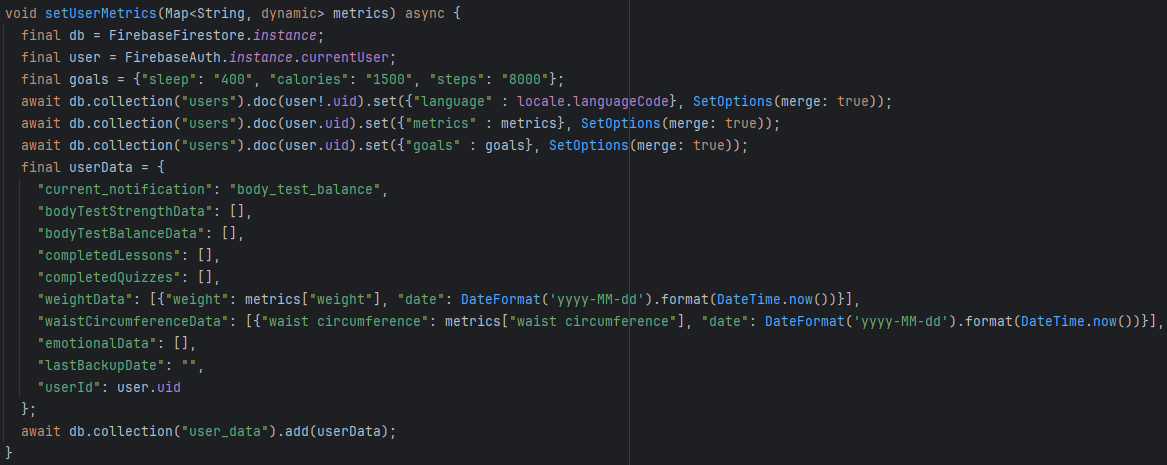
\includegraphics[width=1.0\linewidth]{./images/onBoarding.png}
    \caption{Function Called at the end of the onBoarding process to setup all the needed documents/fields for the user.}
\end{figure*}

\noindent Only the goals are not asked to be inserted in the onBoarding process to avoid make it too long and boring. They have a default value and can be edited in the personal information page at any time.
\newpage

\subsection{State Handling}
All the mobile application states are kept in a class called \texttt{HomeDataProvider} that extends the \texttt{ChangeNotifier}, implementing the best practises regerding the flutter state management and allowing the interface to be updated accordingly whenever some state changes. It is instantiated at the root level of the application with the \texttt{ChangeNotifierProvider} widget that creates a \texttt{ChangeNotifier} and passed down to all the widgets that need to access the data. These widgets can easily access the shared instance by using a \texttt{Consumer} widget, that consumes the above \texttt{ChangeNotifierProvider} allowing to access the instance as well as the context and child. All the relevant states, including the ones to populate the charts (both coming from health as data source or the database) were kept in this class, ensuring a clean state management and an organized code.
\vspace{10ex}
\begin{figure*}
    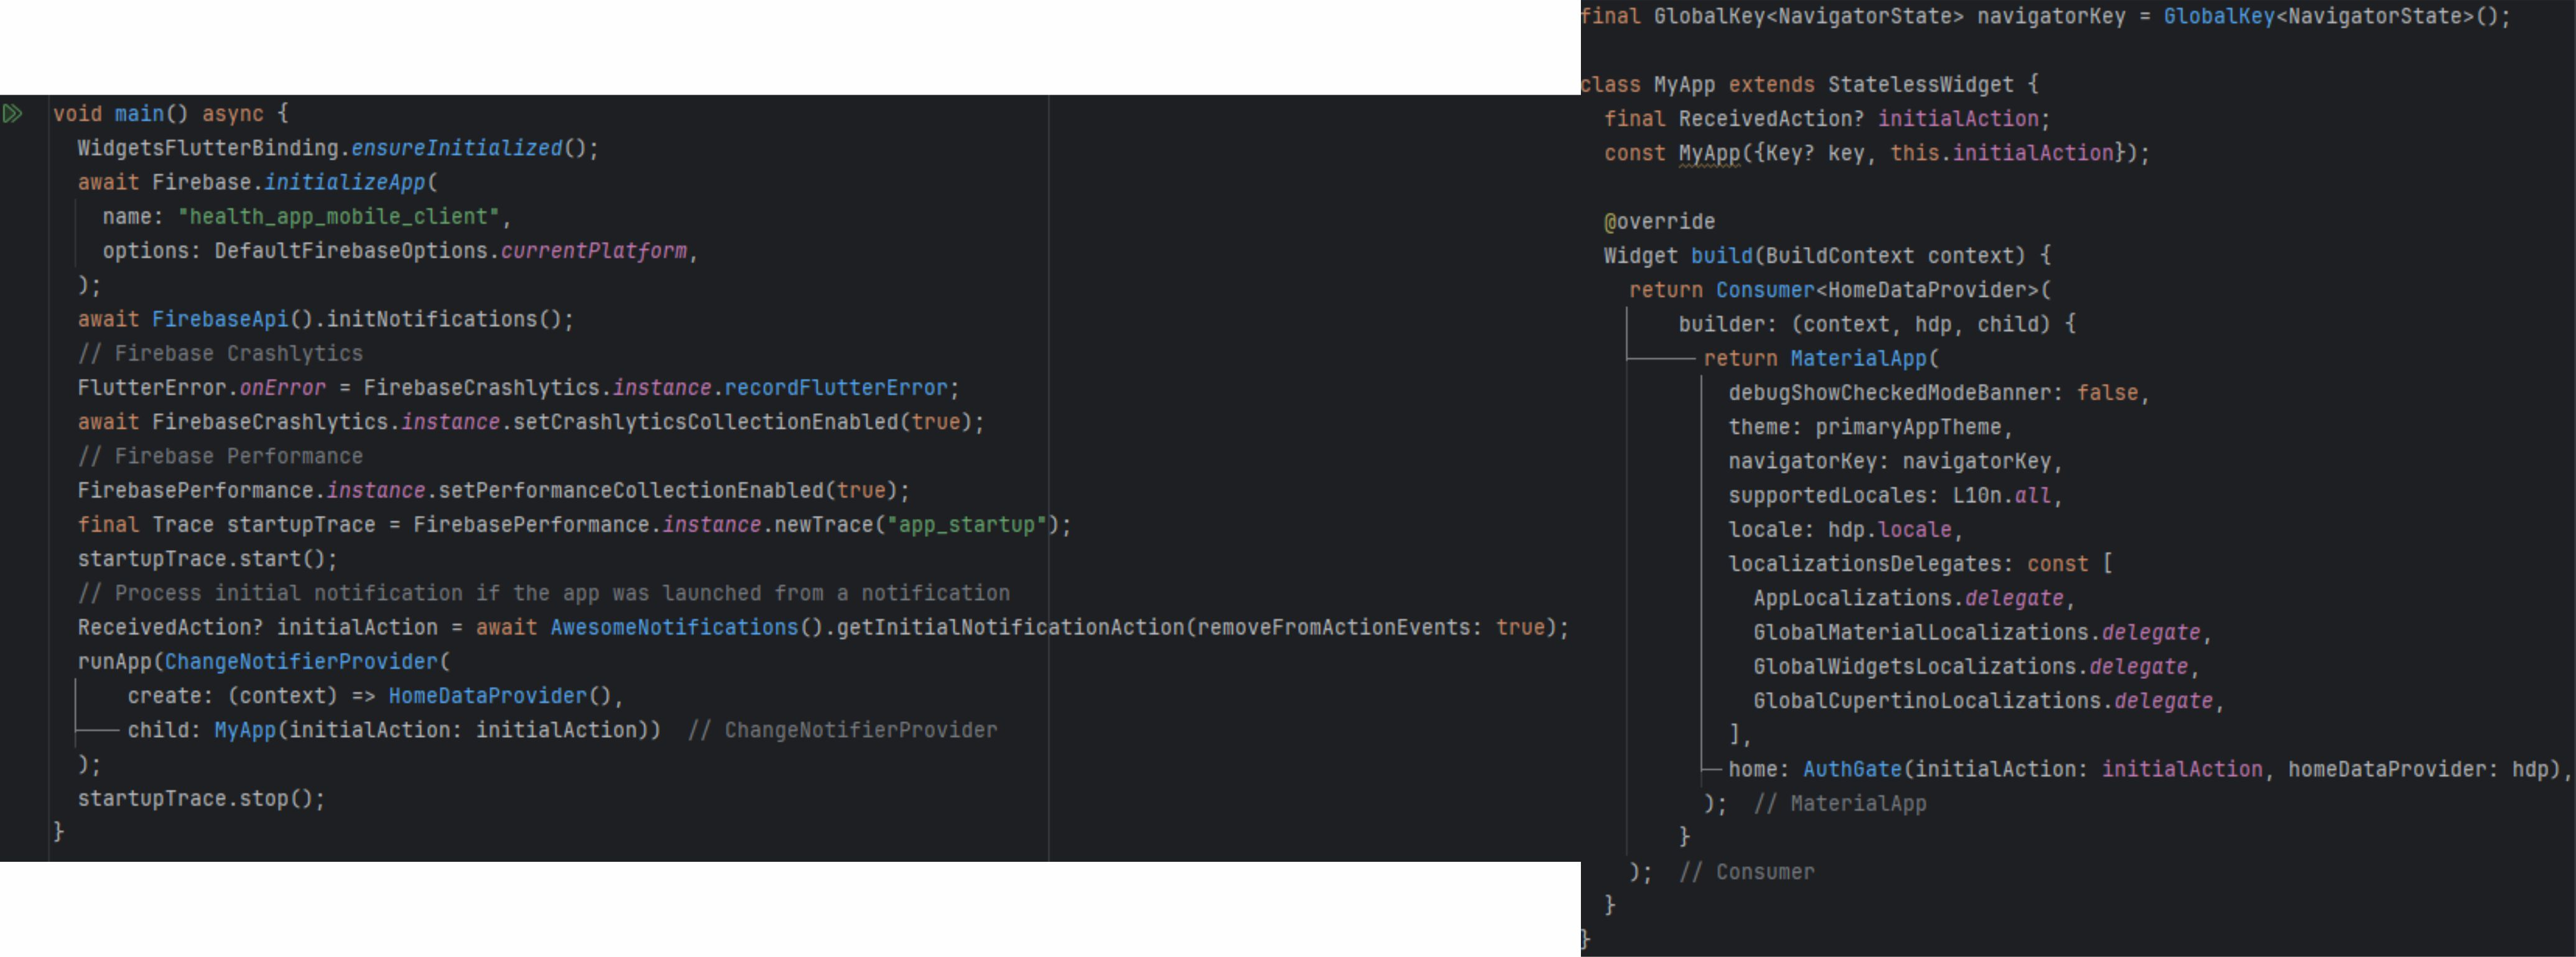
\includegraphics[width=1.0\linewidth]{./images/provider.jpg}
    \caption{HomeDataProvider instantiation at the root level of the app (left) and example of accessing the instance (right).}
    \label{fig:rootHdp}
\end{figure*}
\newpage
\subsection{Home Page}
The home page of the application was designed by allowing the user to have access to his steps, food, sleep and mood data, in which both the database and the health data sources have been employed. While health data are already gathered by the phone/wearable device and provided (is the case of steps and sleep), for food and mood there is also the possibility to let the user insert the data. Considering this aspect, for food and mood the database has been employed as data source instead. Also a \texttt{DateBar} component is present in this page as an utility component, easily allowing to change the selected date, as well as the time period (day,week,month) and view the corresponding data.
\subsubsection{Health Data Source}
As said before, for steps and sleep data, the health data source has been employed. For steps and sleep data, two different states are kept as lists. When, through the health package, the data are retrieved based on the selected date these states are set, and the charts are updated and populated accordingly. For these two metrics, also a chart threshold is set through the users goals, so that the user can see if he is reaching his goals or not. In case the goal is met or also surpassed, the bar appear yellow and with a dotted border, so that the user can easily see the difference. 

\subsubsection{Database Data Source}
For food and mood data instead the database has been employed. However the approach is still the same, except for the data source: two list states are kept, data are fetched also based on the date and chart are updated. In case of food data the threshold like steps and sleep is available. For both food and mood, the user can insert the data through the app with dedicated forms. In case of food, the user can insert the food group and the amount, while for mood the user can insert the positive and negative mood values, according to the PANAS scale. The employed collection are the \texttt{foodRecords} for food and the \texttt{emotionalData} array field into the \texttt{user\_data} collection for mood.
\clearpage
\begin{figure*}
    \centering
    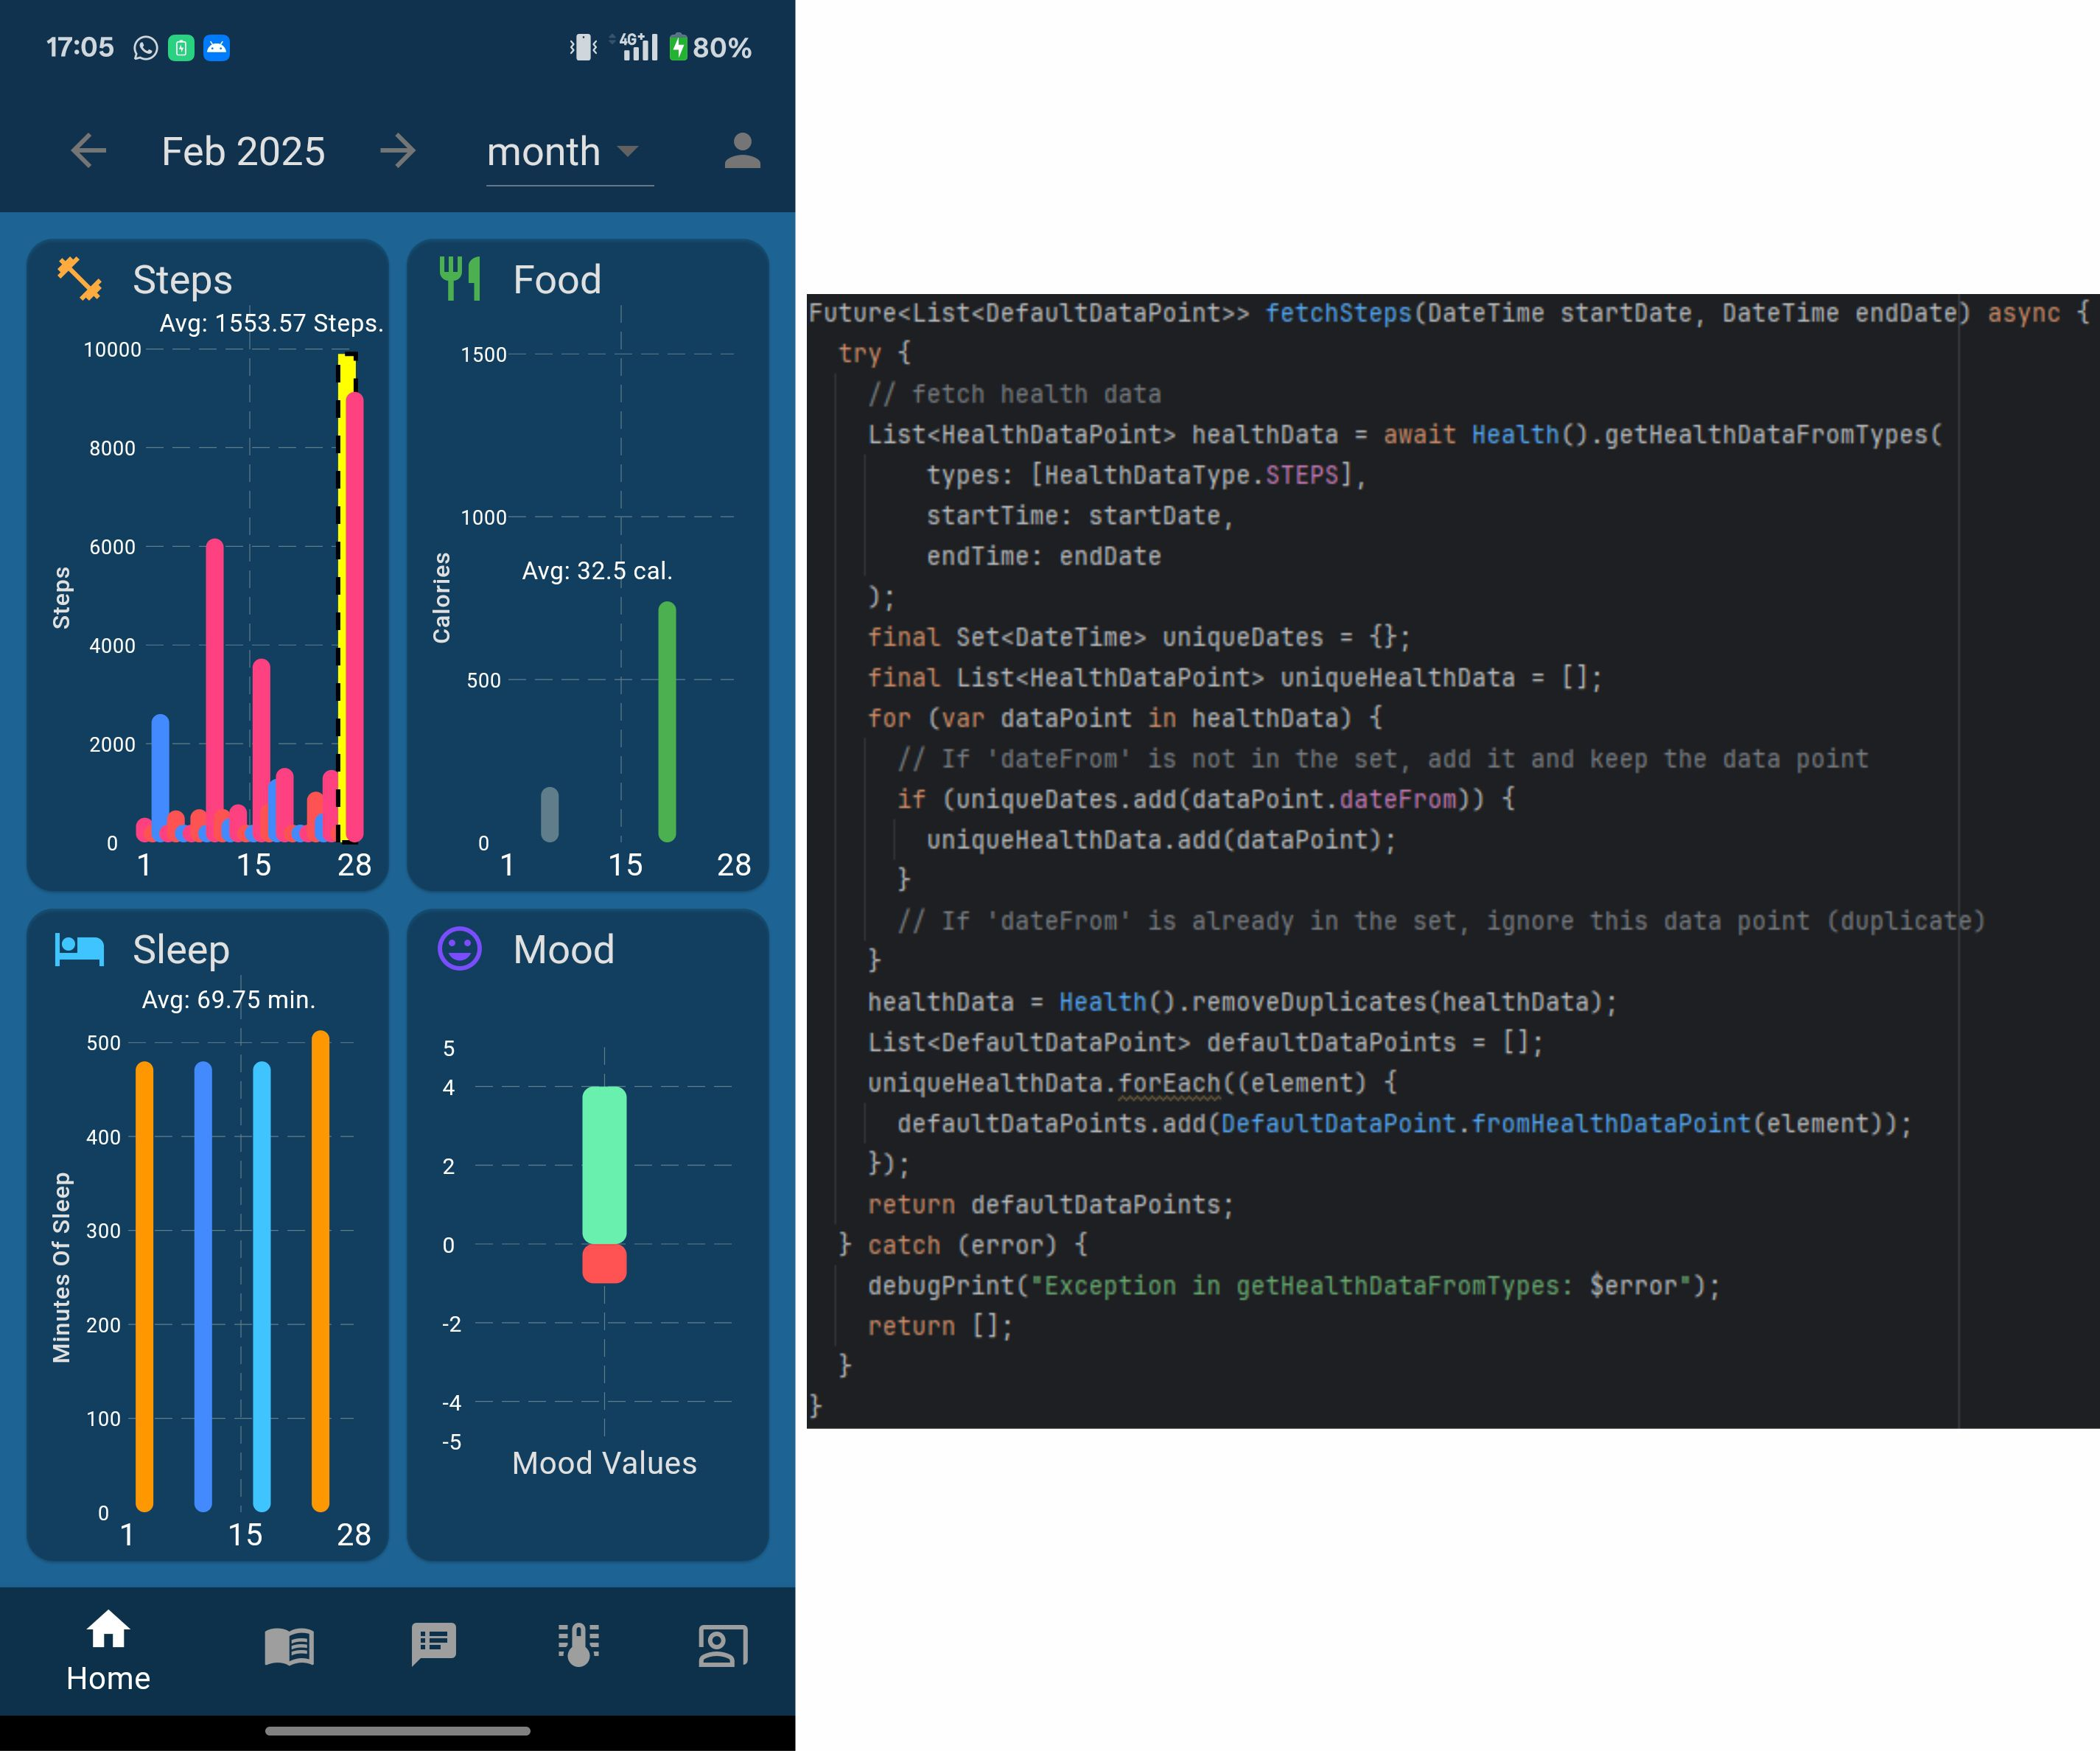
\includegraphics[width=0.7\linewidth]{./images/homeFetch.jpg}
    \caption{Home Page charts (left) and example of health data fetch for the steps (right).}
\end{figure*}

\begin{figure*}
    \centering
    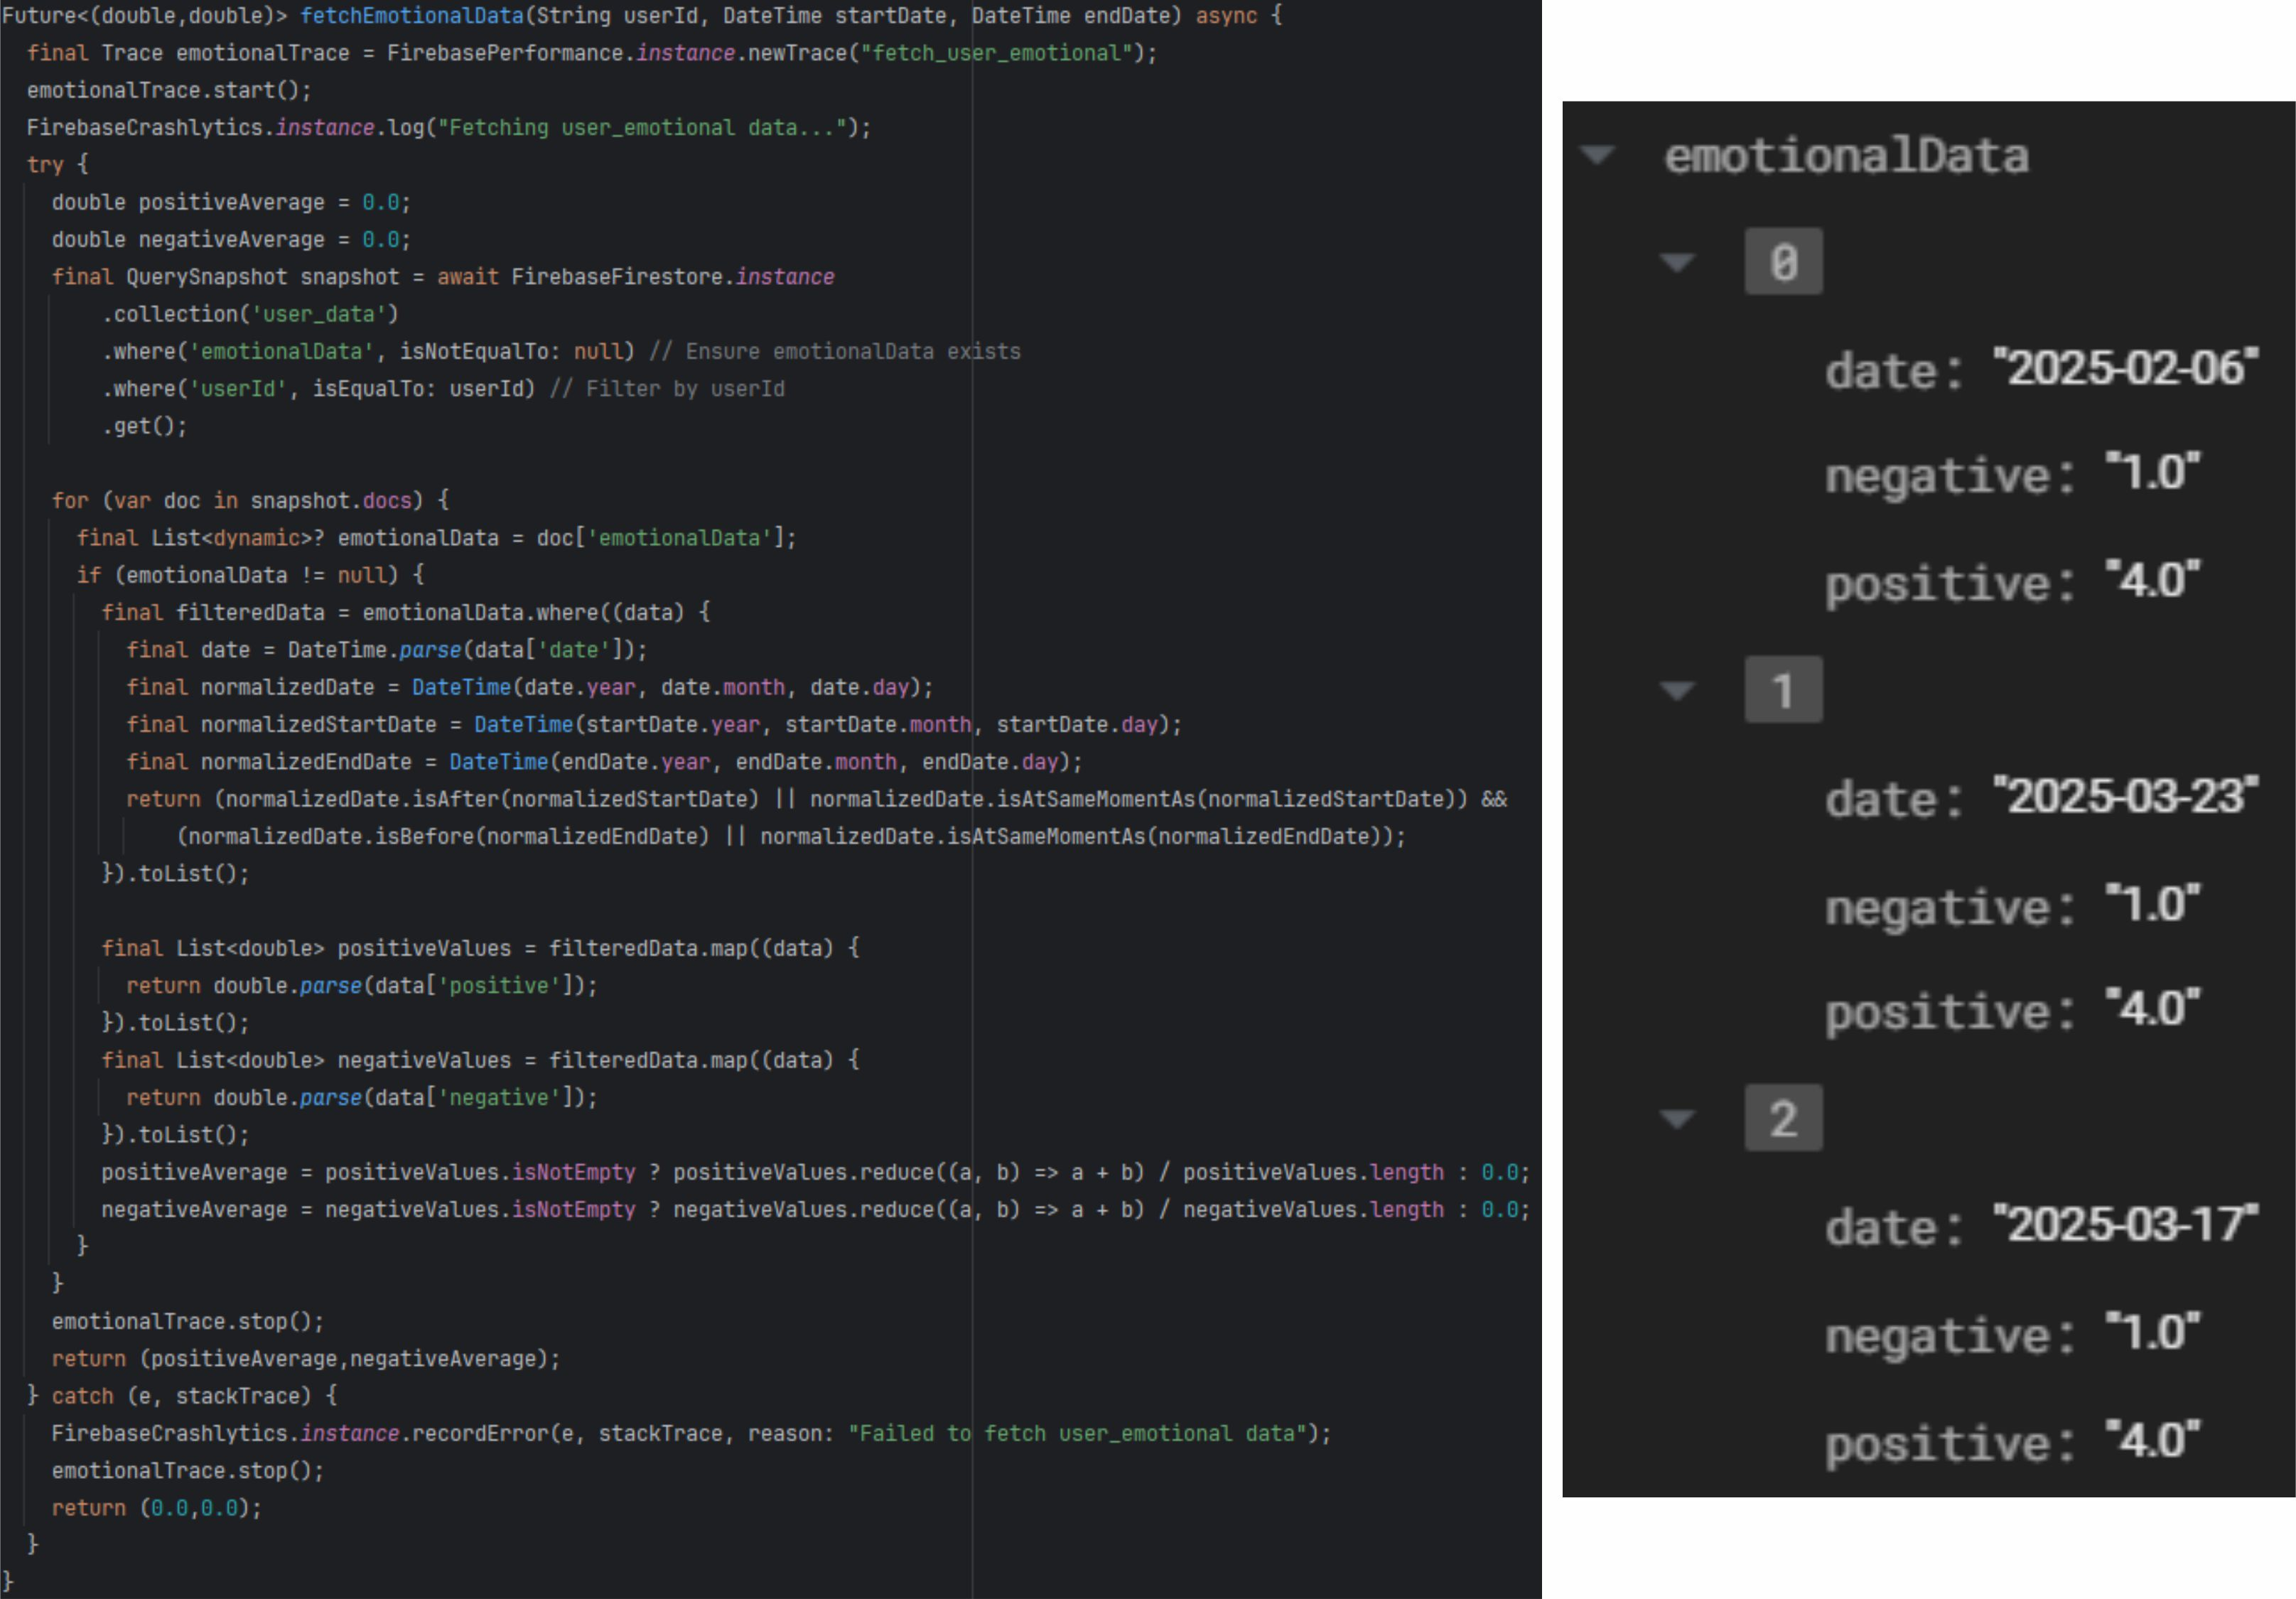
\includegraphics[width=0.7\linewidth]{./images/emotionalFetch.jpg}
    \caption{Example of database data fetch for the emotional data (left) and corresponding database field (right).}
\end{figure*}

\noindent In the steps chart we can also see the overflow of the related goal in one particular day that makes the bar appear differently.

\subsection{Health Measures Page}
In the health measures page the user can see additional data about his health. \newline A tab subdivision has been made to obtain a clearer view of the data:
\begin{itemize}[nosep] % 'nosep' removes extra spacing between items
    \item \textbf{Lungs-related data tab}, composed of:
    \begin{itemize}[nosep]
        \item Oxygen Saturation chart, representing the oxygen saturation in the blood.
        \item Respiratory Rate chart, representing the number of breaths per minute.
    \end{itemize}
    \item \textbf{Heart-related data tab}, composed of:
    \begin{itemize}[nosep]
        \item Resting Heart Rate chart, useful health metrics, measured in breaths per minute.
        \item Heart Rate Variability chart, representing the variation in time between heartbeats.
    \end{itemize}
    \item \textbf{Body-related data tab}, composed of:
    \begin{itemize}[nosep]
        \item Weight chart, measured in kilograms.
        \item Waist Circumference chart, mesured in centimeters.
        \item Body Balance chart, composed of the left leg, right leg and tandem walk tests, all measured in seconds.
    \end{itemize}
    \item \textbf{Strength-related data tab}, composed of:
    \begin{itemize}[nosep]
        \item Grip Strength chart, measured in kilograms.
        \item Waist Circumference chart, mesured in centimeters.
        \item Body Strength chart, composed of the abs count, push up count and squat count, all measured in repetitions.
    \end{itemize}
\end{itemize}
Also here the \texttt{DateBar} component is present in this page to change the selected date, as well as the time period (day,week,month) and view the corresponding data.
\subsubsection{Health Data Source}
For the first two tabs (lungs and heart), the health data source has been employed. All these data are directly retrieved through the health package, similarly to the home page steps data. We have four list states (currentOxygenDataPoints, currentBreathRateDataPoints, currentHeartRateDataPoints and currentRestingHeartRateDataPoints) that are set when the data are retrieved based on the selected date. Also in this case, the charts who depend on these states are updated and populated accordingly.

\subsubsection{Database Data Source}
For the last two tabs instead (body and strength), the database has been employed, particularly the \texttt{user\_data} collection, that contains the array fields \texttt{weightData},\newline\texttt{bodyTestBalanceData}, \texttt{waistCircumferenceData} and \texttt{bodyTestStrengthData}. Except for the data source the approach is still the same: four list states (currentWeightDataPoints, currentWaistCircumferenceDataPoints, currentBodyBalanceDataPoints and currentBodyStrengthDataPoints) are kept, data are fetched similarly to the emotional data (also stored on database) based on the date and charts are updated. In this case however, the user has the possibility to insert also the data with dedicated forms, giving the possibility to have an hystorical view of metrics like weight and understand eventual improvement or worsening.

\begin{figure*}
    \centering
    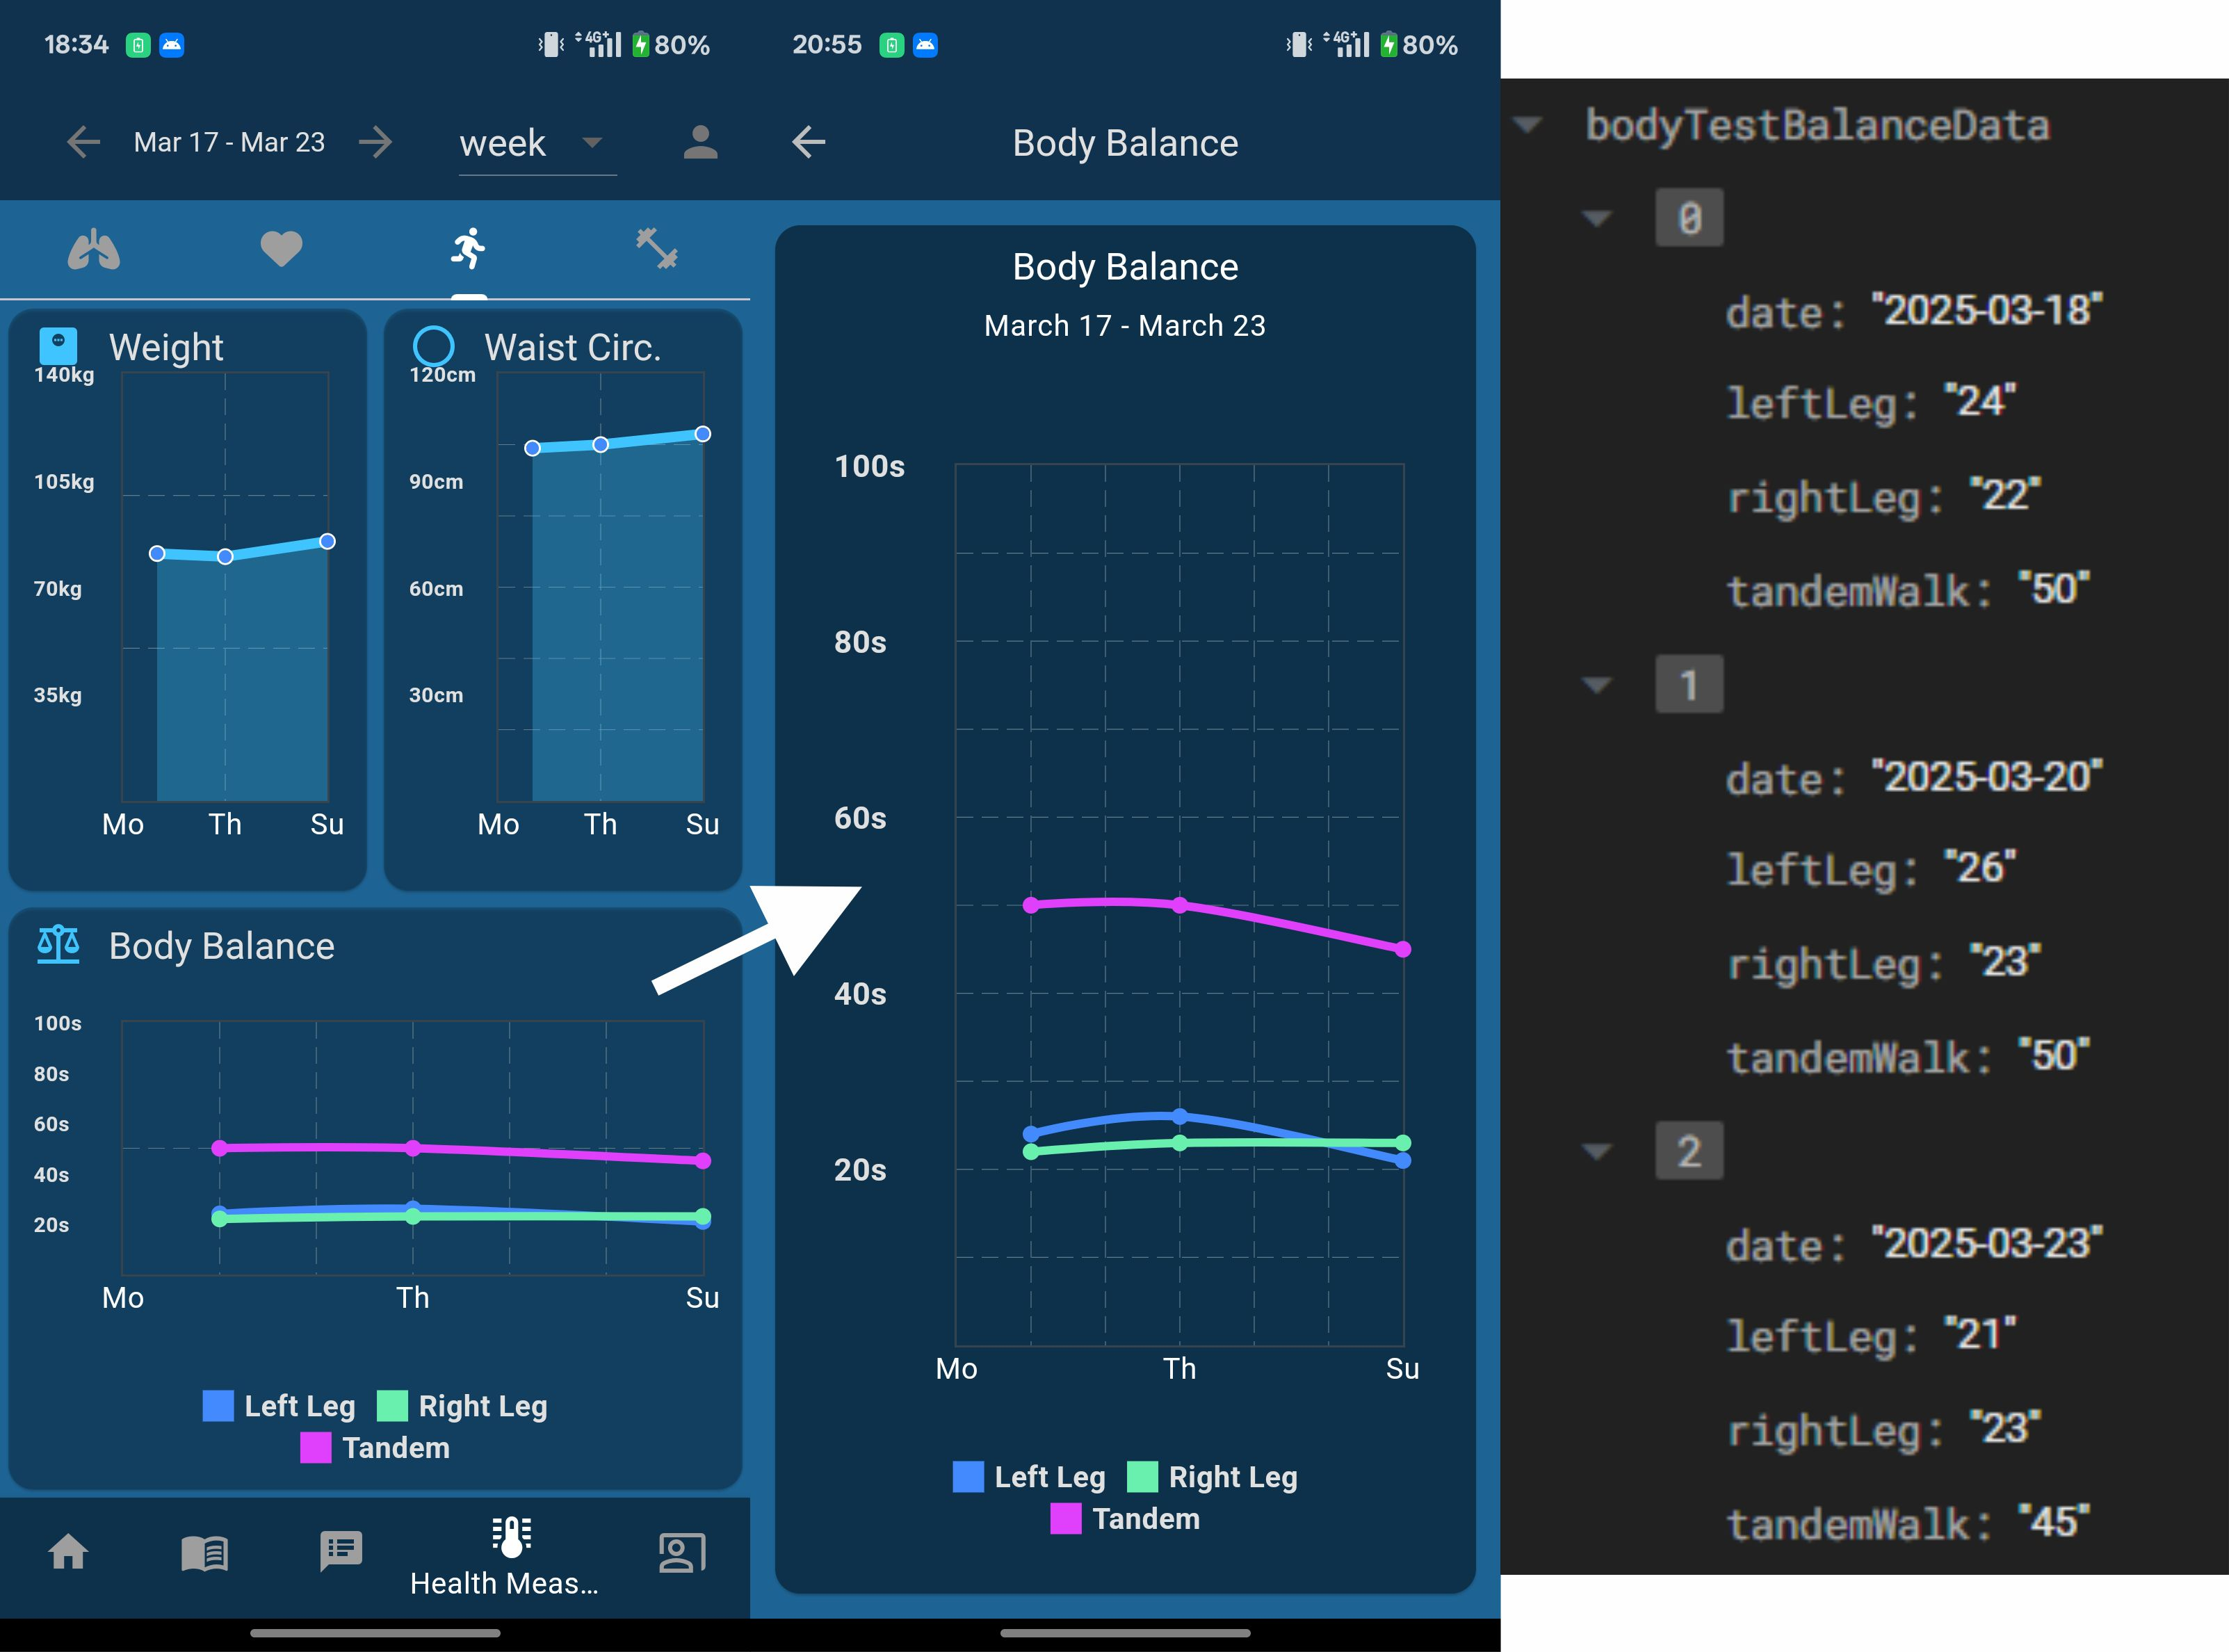
\includegraphics[width=1.0\linewidth]{./images/healthMeasures.jpg}
    \caption{Health Measures Page on Body-related data tab (left), detailed view of the Body Balance chart (center) and his corresponding database field (right).}
\end{figure*}

\subsection{Personal Information Page}
In this page the user has the possibility to edit part of his metrics as well as editing his goals. Since those metrics are acquired in the onBoarding phase, they are all handled through the database and stored in the user-generated document inside the \texttt{users} collection, in particular in the \texttt{metrics} field.
\newline Also in this case in order to have a clearer view of the data there is a tab split into:
\begin{itemize}[nosep] % 'nosep' removes extra spacing between items
    \item \textbf{Personal Measures tab}, composed of almost all the users metrics. Metrics not present in this page are the weight and the waistCircumference, since they can be added in the healthMeasures page, where in addition the historical view of these data is displayed. The present metrics are freely editable at any time after user registration, except for the birthDate, only displayed for obvious reasons.  
    \item \textbf{Goals tab}, composed of the users goals, freely editable at any time after user registration. The goals are used to set the threshold of the charts in the home page, so that the user can see if he is reaching his goals or not.
\end{itemize}

\begin{figure*}
    \centering
    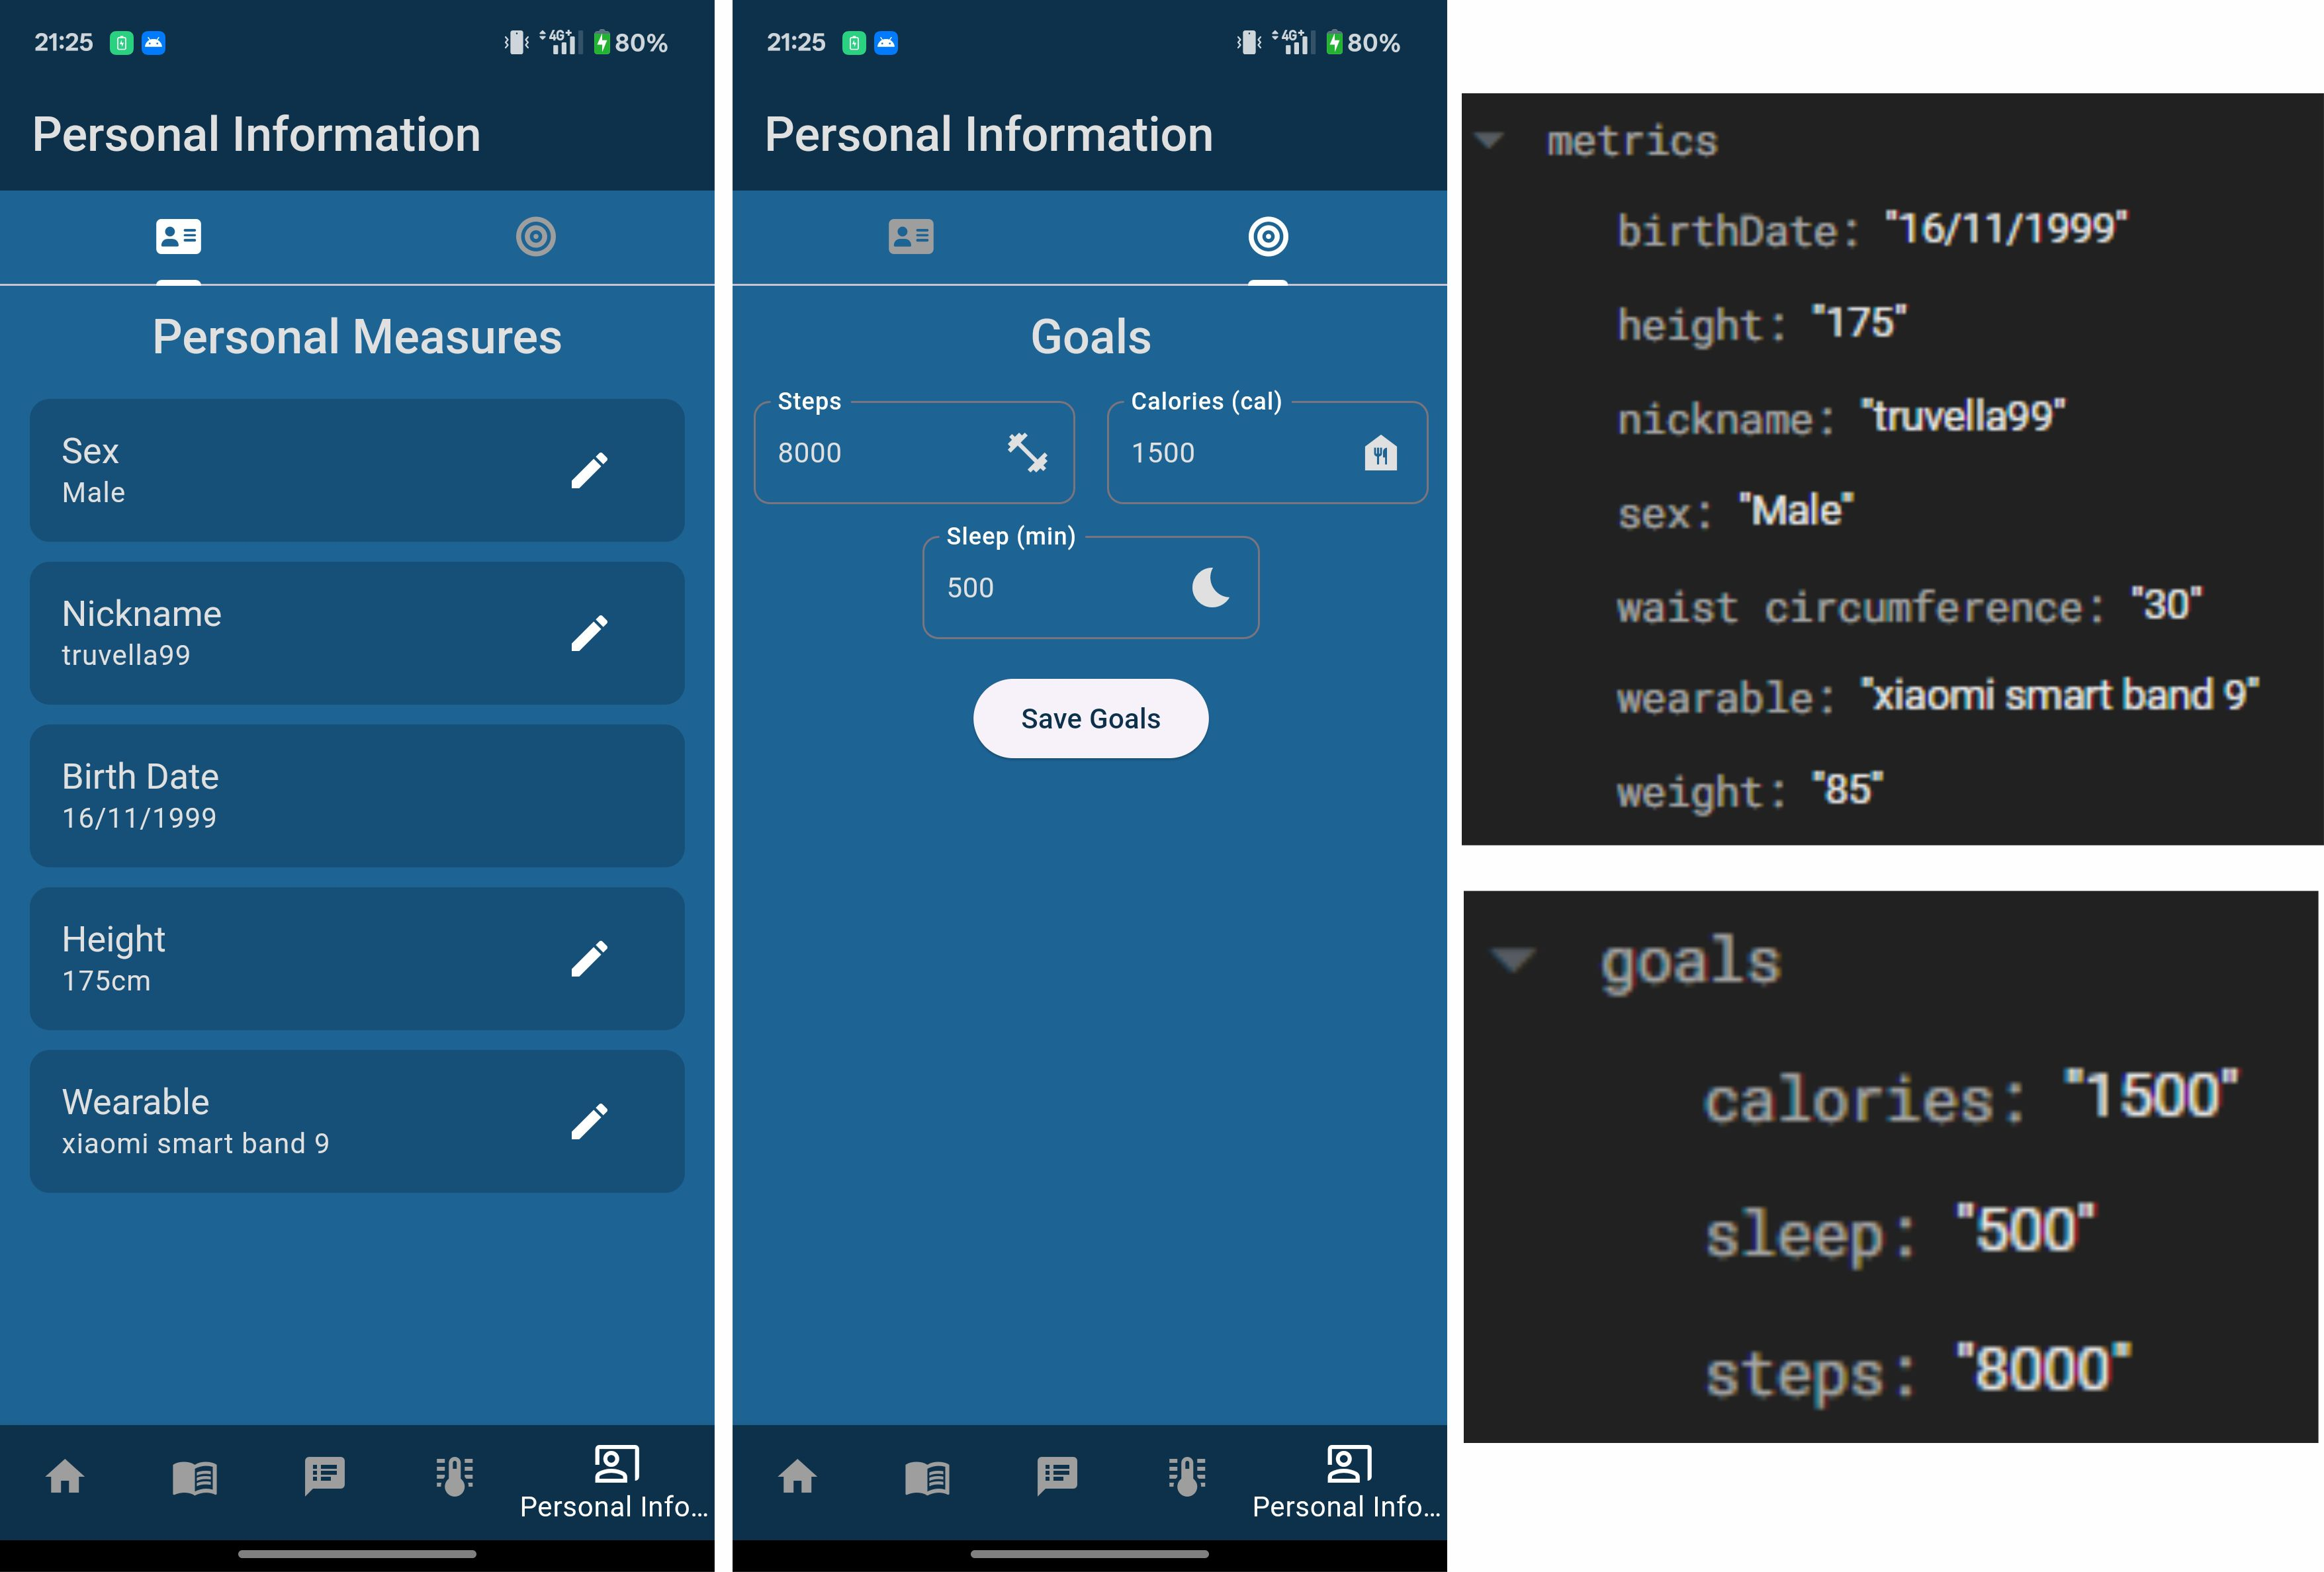
\includegraphics[width=0.7\linewidth]{./images/personalInformation.jpg}
    \caption{Personal Information Page with Personal Measures tab (left), Goals tab (center) and corresponding database field (right).}
\end{figure*}

\noindent Both the metrics and goals are updated in the database when the user changes them by using the \texttt{SetOptions(merge: true)} method, so that only the fields that are changed are updated and not the whole document.
\subsection{Learn Page}
In the learn page the user has the possibility to browse the available lessons and learn new things. The lessons and quizzes are managed through the \texttt{lessons} and the \texttt{quizzes} collection, where the single lesson references the quiz through the \texttt{quizId} field. Other additional fields are also used to store information of the single user. Infact, each lesson is composed of several pills, and the \texttt{completedPills} field is employed (see \cref{subsubsec:completedPills}): when the user reads a certain pill of a lesson, the corresponding array field is updated with a true value, with an index correspondance between the pill and the boolean field in the array. In this way the user can see how many pills of a lesson he has read and how many are still to read, and only when all the pills have been read the whole lesson is marked as read. Regarding the quiz instead, to leave the user with more freedom, it can be taken at any time, but the quiz is marked as completed (the quizId is added to the \texttt{completedQuizzes} array field still in \texttt{user\_data}) only if the user completes it with success. Both lessons and quizzes supports localization and have their italian traslation stored in the \texttt{pillsIta} and \texttt{questionsIta} fields respectively. The user will be able to see this version by changing the default language of the app.
\begin{figure*}
    \centering
    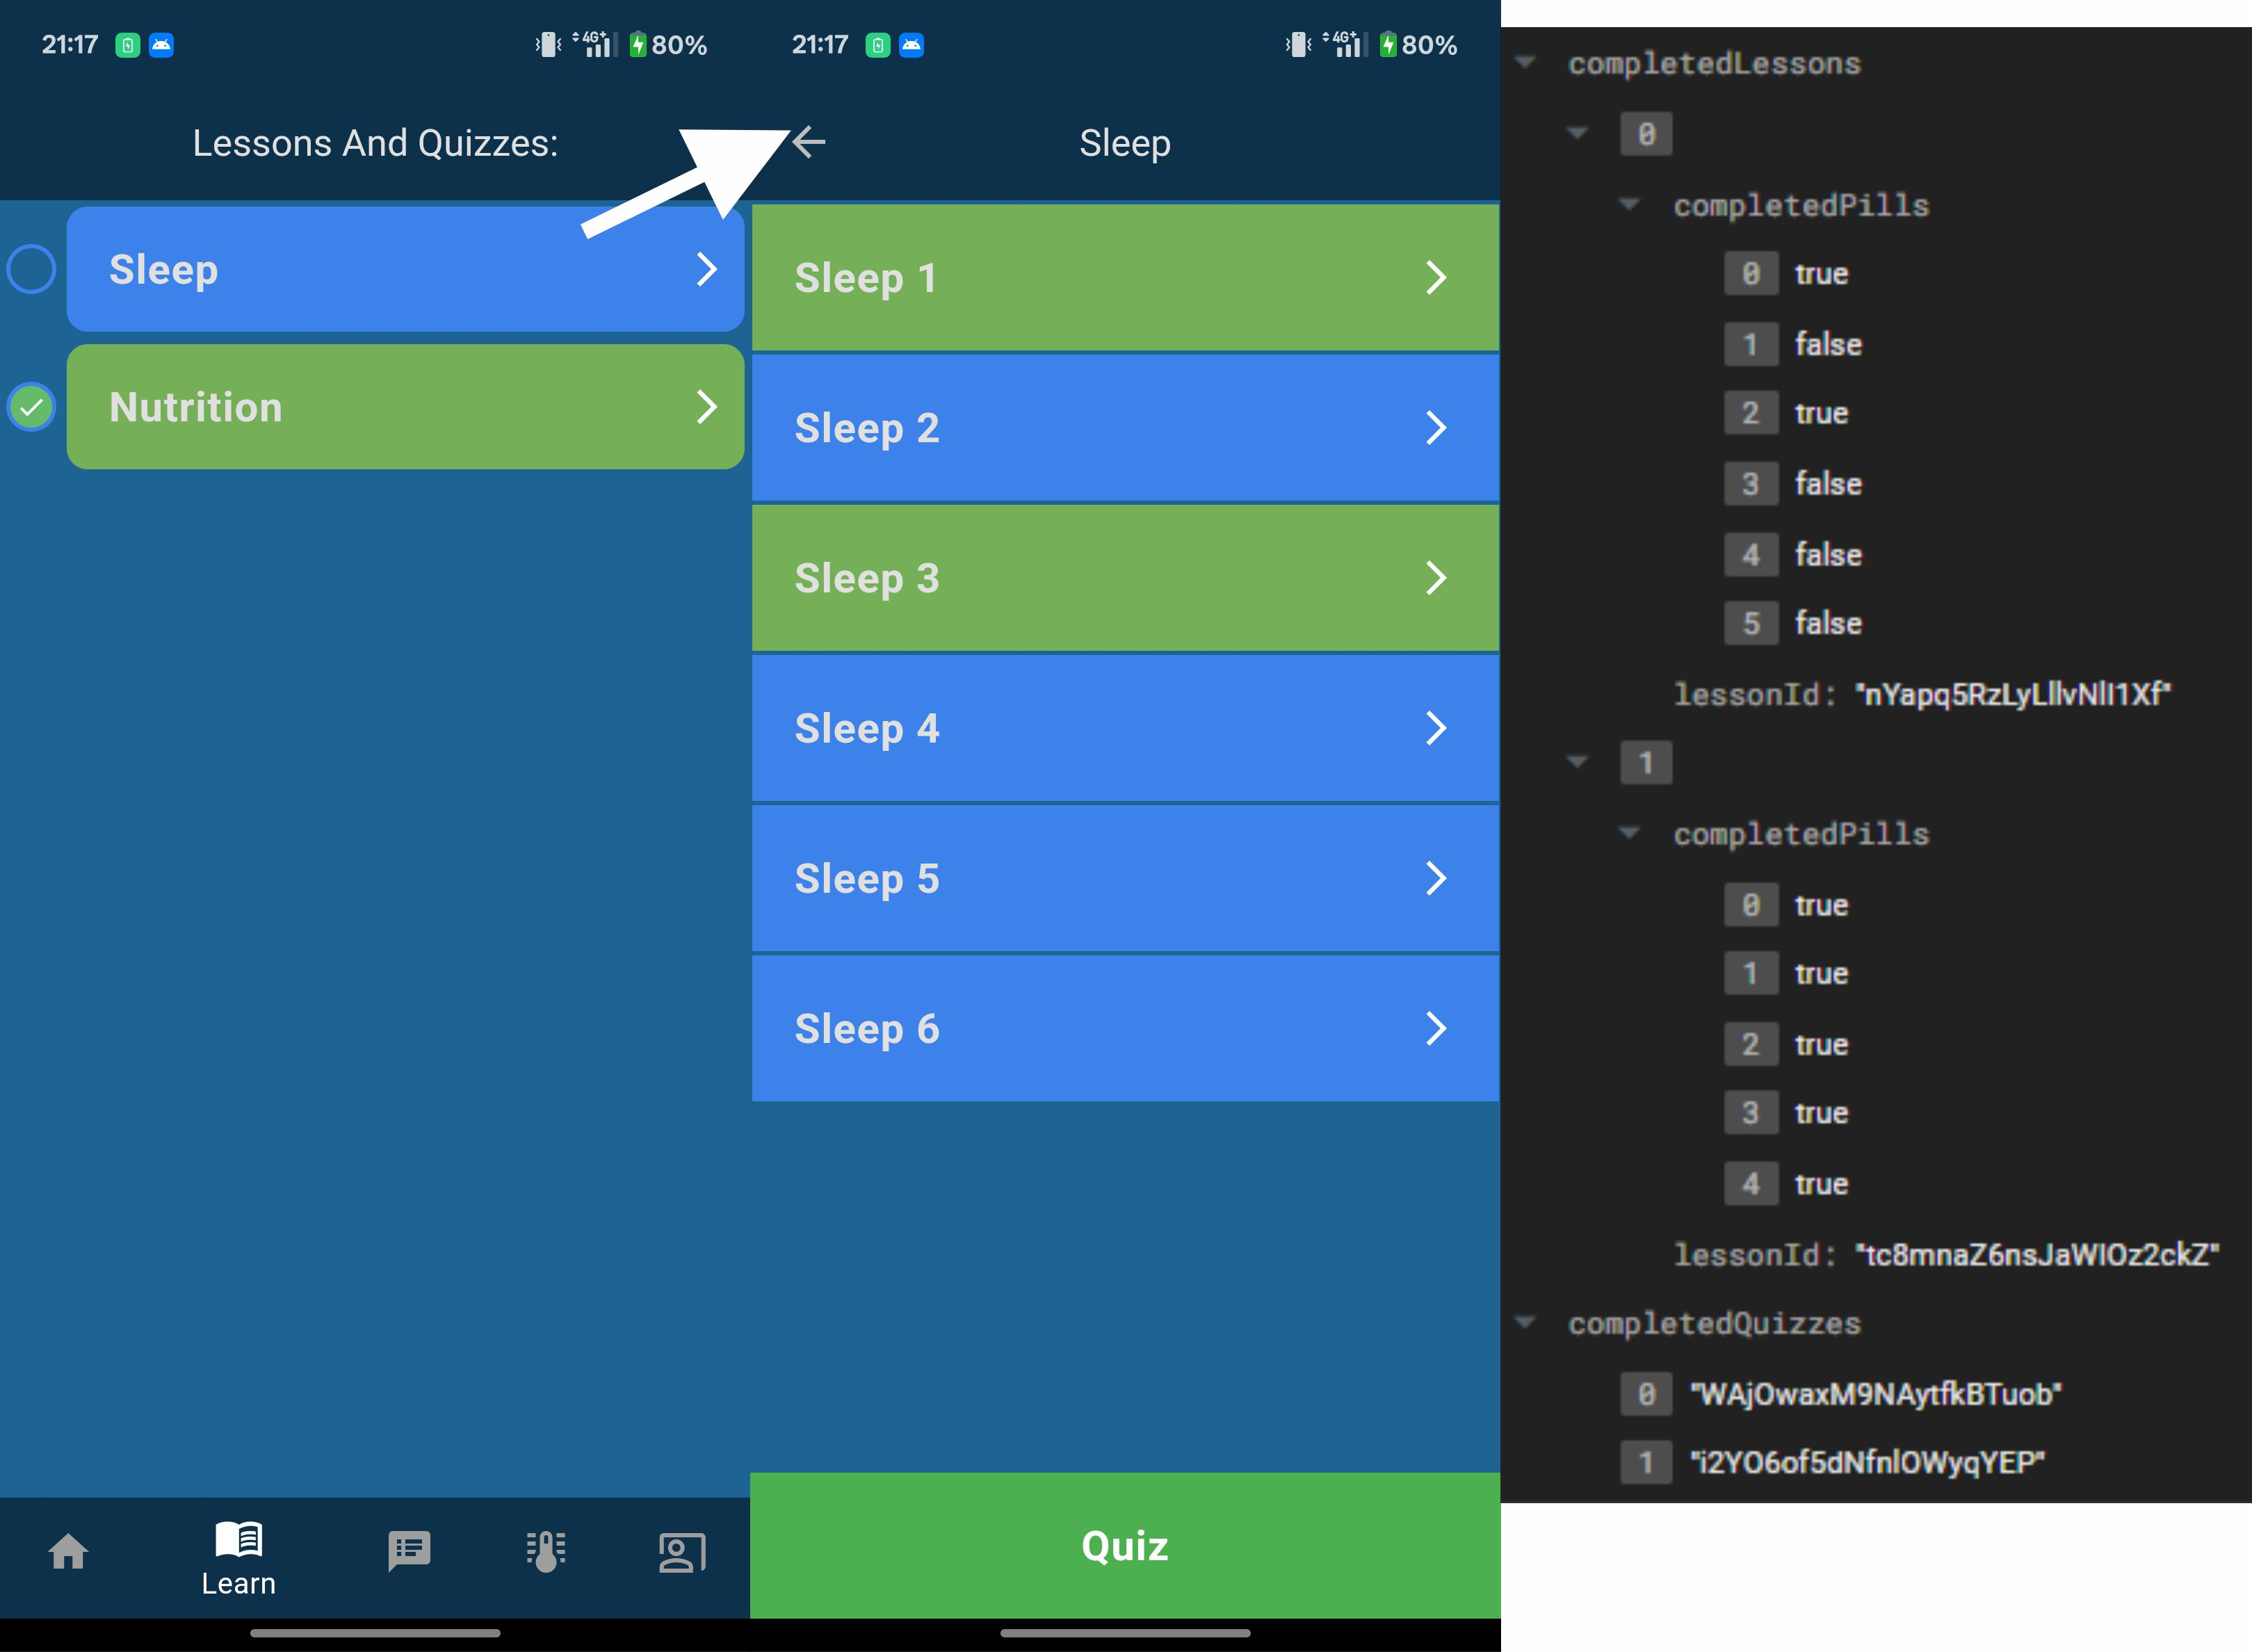
\includegraphics[width=0.6\linewidth]{./images/lessonsQuizzes.jpg}
    \caption{User View of the Lessond and Quizzes (left), of e lesson in detail (center) and the database fields to handle pills reading (right).}
\end{figure*}

\noindent In this example we can see the pills handling, since for the sleep lesson only pills 1 and 3 are read (same array fields set to true), while for the nutrition lesson all the pills are read. Both quiz however are completed and added to the \texttt{completedQuizzes} field.
\subsection{MultiLanguage}
Also the multilanguage feature has been implemented, in order to satisfy the localization requirement (see \cref{tab:nfr} NFR8). Implementing this feature required additional fields on the database, as well as additional management on the application side. 
As explained previously (see \cref{subsubsec:cloudFirestoreDatabase}) an additional field was added for each user document inside the \texttt{user\_data} collection called \texttt{language}, used to store the current language selected by the user (english by default). Also other fields were added to handle multilanguage: for the lessons and quizzes the \texttt{pillsIta} and \texttt{questionsIta} fields were added, while for the notifications an additional document in the \texttt{notifications\_text} collection was employed, that contains the italian version of the parameters. The user will be able to see either the english or italian version by changing the default language of the app through a dropdown on the top right of the screen (see \cref{fig:authenticationScreens} middle image), and changing his \texttt{language} value will imply a change of the whole app language. 
\newline As application side setup, the \texttt{l10n.yaml} file and \texttt{l10n} folder were created. The first file was used to configure the default directory where the \texttt{.arb} files (traslation files) will be stored (the \texttt{l10n} directory), as well as the default traslation file to pick (\texttt{app\_en.arb}) and the output \texttt{.dart} file that contains the localization code. This because running the build with all the files configured will produce auto-generated locale output \texttt{.dart} files for all supported locales, that can be imported and then used. Inside the \texttt{l10n} folder the \texttt{l10n.dart} file was defined, which contains a class with an array field named \texttt{all}, containing all the supported locales (only en for english and it for italian), as well as the traslation files (\texttt{app\_en.arb} and \texttt{app\_it.arb}) that contains the traslation of the app strings in the two languages.
\newline The multilanguage support was handled from the \texttt{MyApp} root component by setting the locale, defined as a HomeDataProvider state that can be changed at any time (see \cref{fig:rootHdp} right side): this allowed to change the language also during the onBoarding process, so that the user can see the app in his preferred language from the beginning, and the language setting persists also after registration.
\newline Once implemented that, all it took was defining the traslation strings in the \texttt{.arb} files with a key/value format, and referring them throughout the whole application. The \texttt{AppLocalizations.of(context)} method was employed to access the traslation strings, allowing to traslate the whole application in the selected language. \newline For example, given the \texttt{learn} key, having value Learn in english and Impara in italian, the \newline\texttt{AppLocalizations.of(context)!.learn} will return Learn or Impara based on the selected language.

\begin{figure*}
    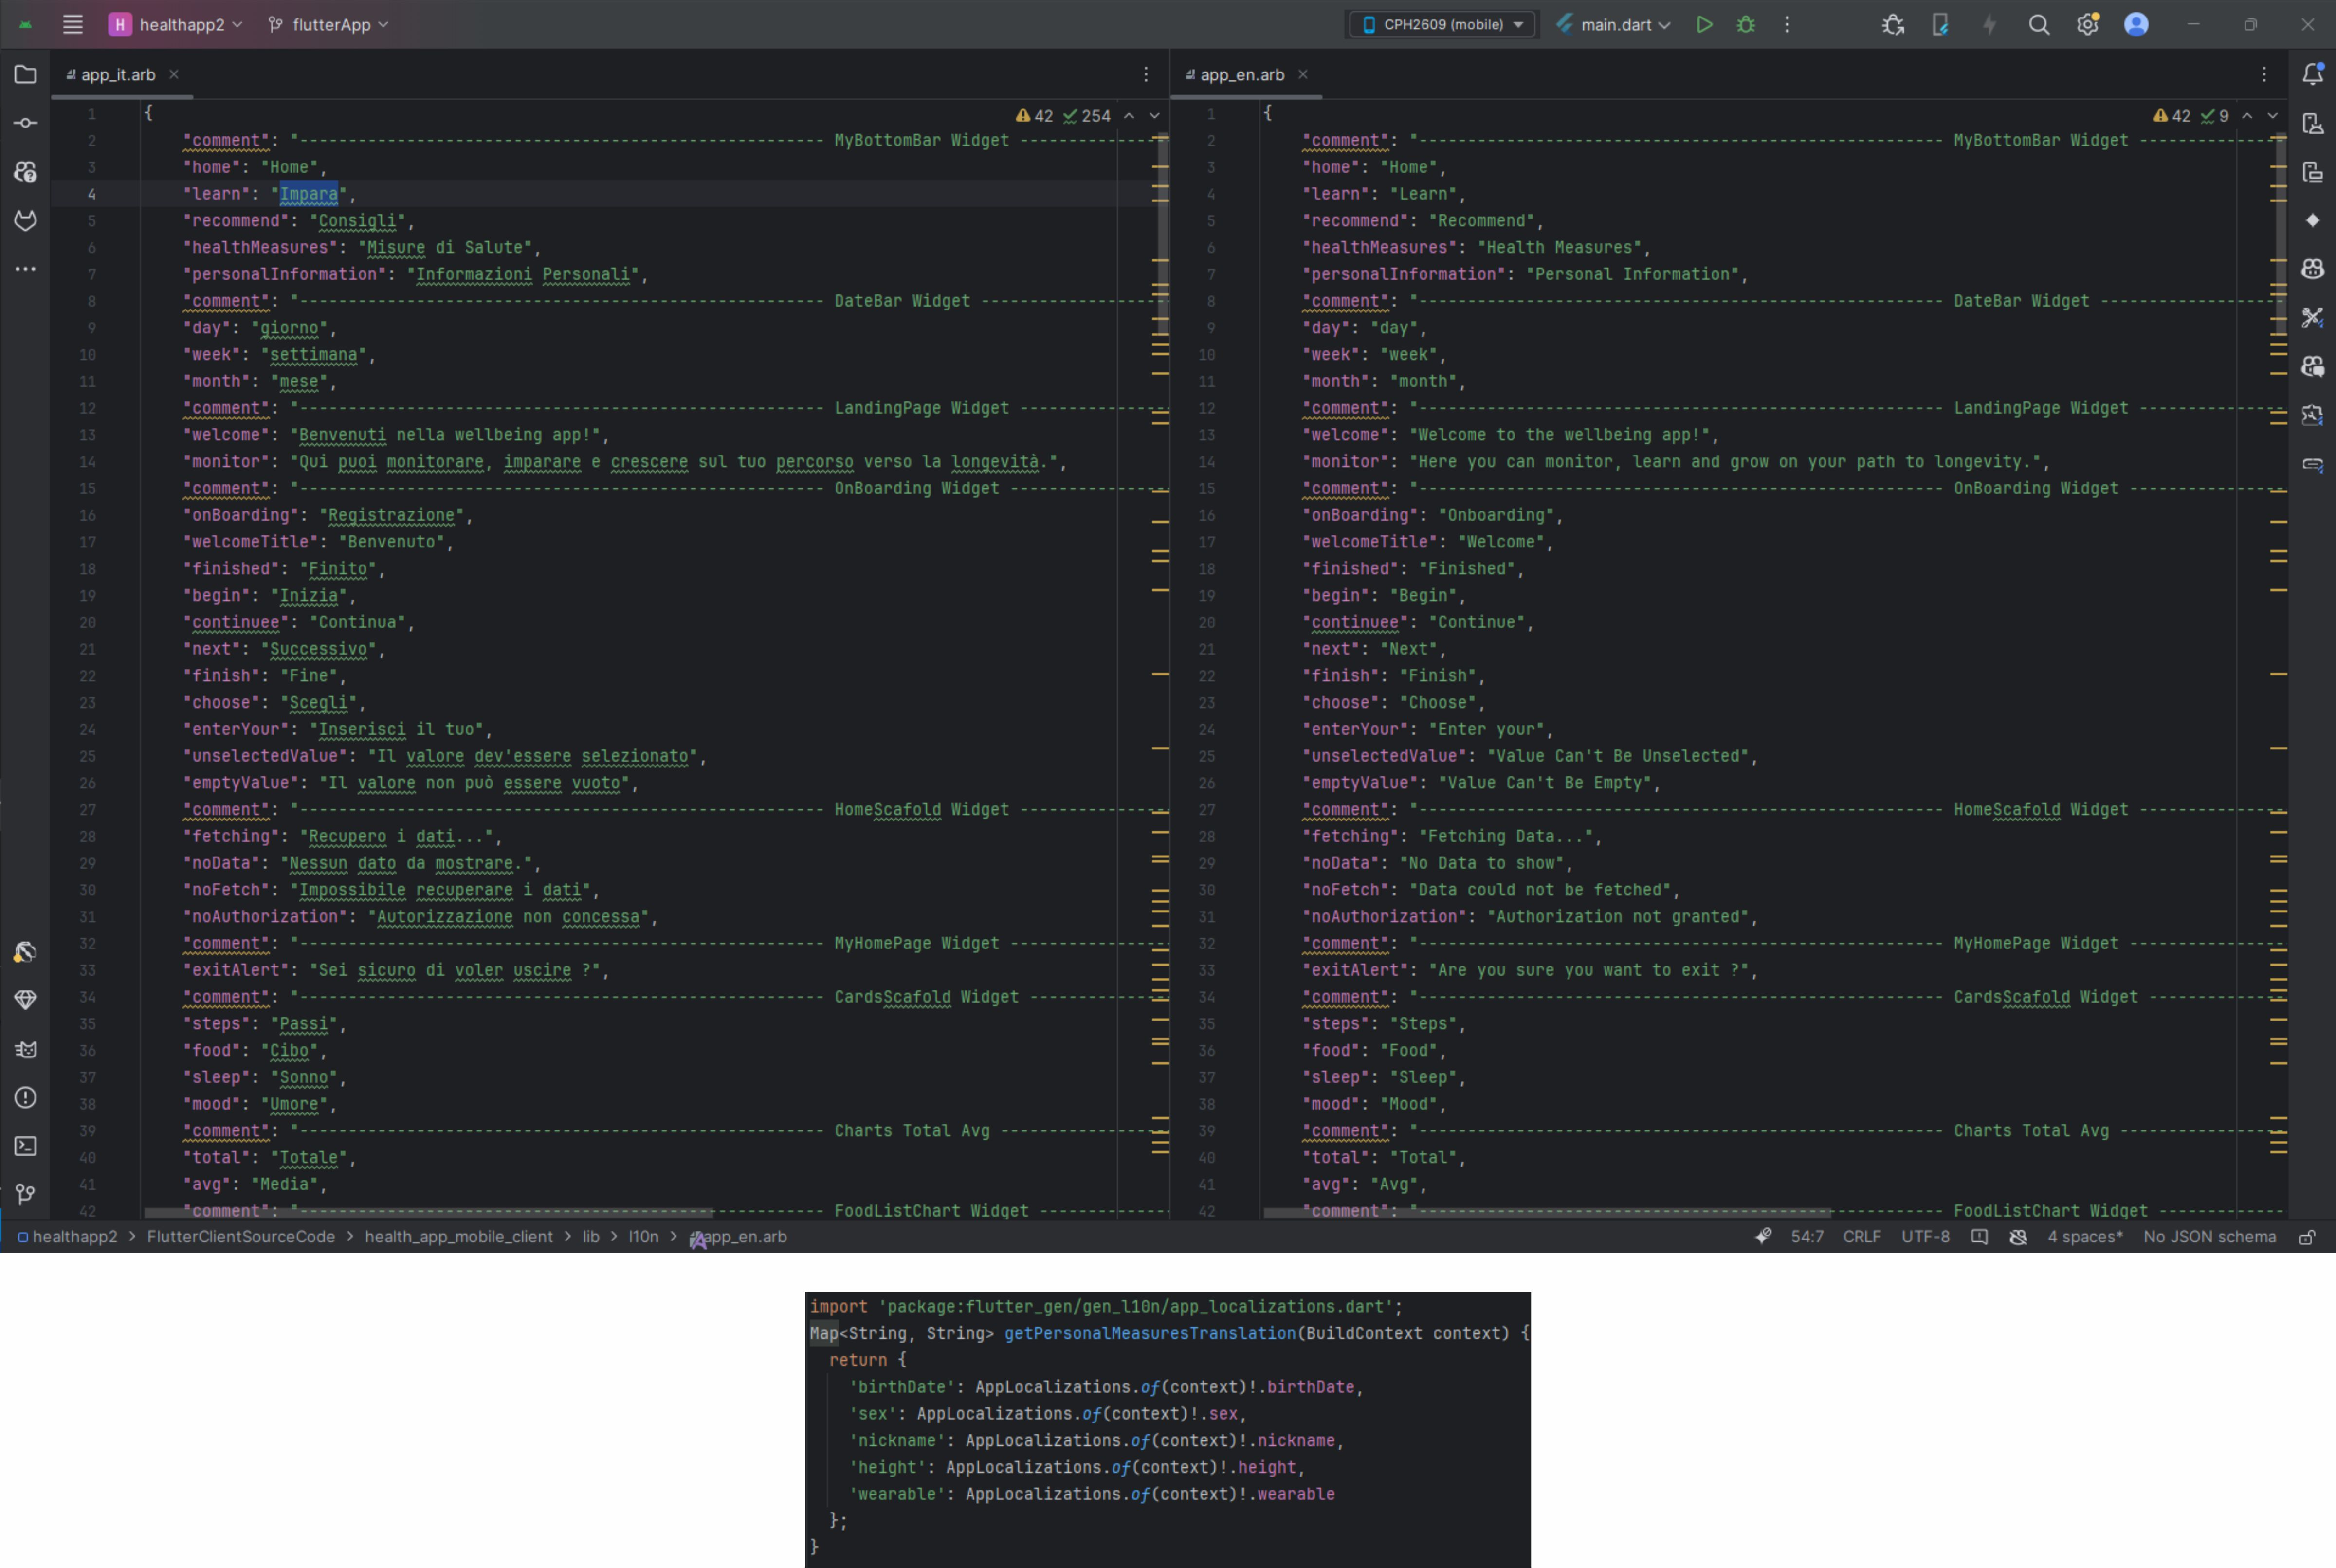
\includegraphics[width=1.0\linewidth]{./images/multiLanguage.jpg}
    \caption{\texttt{.arb} files structure definition (top) and usage example of the multilanguage feature (bottom).}
\end{figure*}

\subsection{Health Data Backup with Cloud Storage}
In order to perform the backup of the health data and satisfy the related requirement (see \cref{tab:fr4}), the cloud storage service has been employed. The main reason lies behind the fact that health data can be pretty large, so using the Cloud Firestore Database to store them would be inefficient and expensive. For this reason the health data are stored on the cloud storage into JSON files, one for each backup. The backup task is performed thanks to the flutter workmanager library by running a background task in background, allowing to execute the backup even if the mobile app is not opened or actively used in that moment. However, since these tasks run on a separate background isolate, retrieving the health data directly there is not possible due to permission issues.
\noindent For this reason, the backup implementation is structured into three phases:
\begin{enumerate}[nosep] % 'nosep' removes extra spacing between items
    \item In the first phase, that takes place at each application startup, the \newline \texttt{performLocalBackup} function is called. This function retrieves the health data in the main isolate (so having the permission) through the health library (starting from the \texttt{lastBackupDate} field taken from the \texttt{user\_data} collection for each user) and stores them into a JSON file in the local storage of the device, named with \texttt{Datetime.now().toIso8601String()} to guarantee univocity. After that the \texttt{lastBackupDate} field is coherently updated to \texttt{Datetime.now()}. This local backup is performed with a daily frequency, so if the app is opened more than once a day or simply no data are available the function returns immediately, to avoid to increase the frequency or to create an empty file.
    \item In the second phase, that takes place immediately after the first one, the workmanager background task is scheduled through the \texttt{scheduleBackupTask} function. The task is a periodic task with the same frequency of the local backup (daily). Also in this case, if the app is opened more than once a day, even if the function is called multiple times, the task id guarantees that the task still is scheduled once.
    \item In the third phase, that takes place when the workmanager background task triggers and is executed, Firebase is initialized in the background isolate and the \texttt{performStorageBackup} function is called. This function loops through the JSON files saved in the local storage of the device and it uploads them to the storage. In case of successful upload, these files are marked for deletion and a second loop proceeds to delete them from the local storage of the phone. In case of failure, the files are not deleted and they will be uploaded when the task will be triggered again. These files are saved on the cloud storage in a folder named with the userID to guarantee univocity and to avoid conflicts between different users' backups, while the filename is also unique, since it is the same that was defined in the \texttt{performLocalBackup} function.
\end{enumerate}

\begin{figure*}
    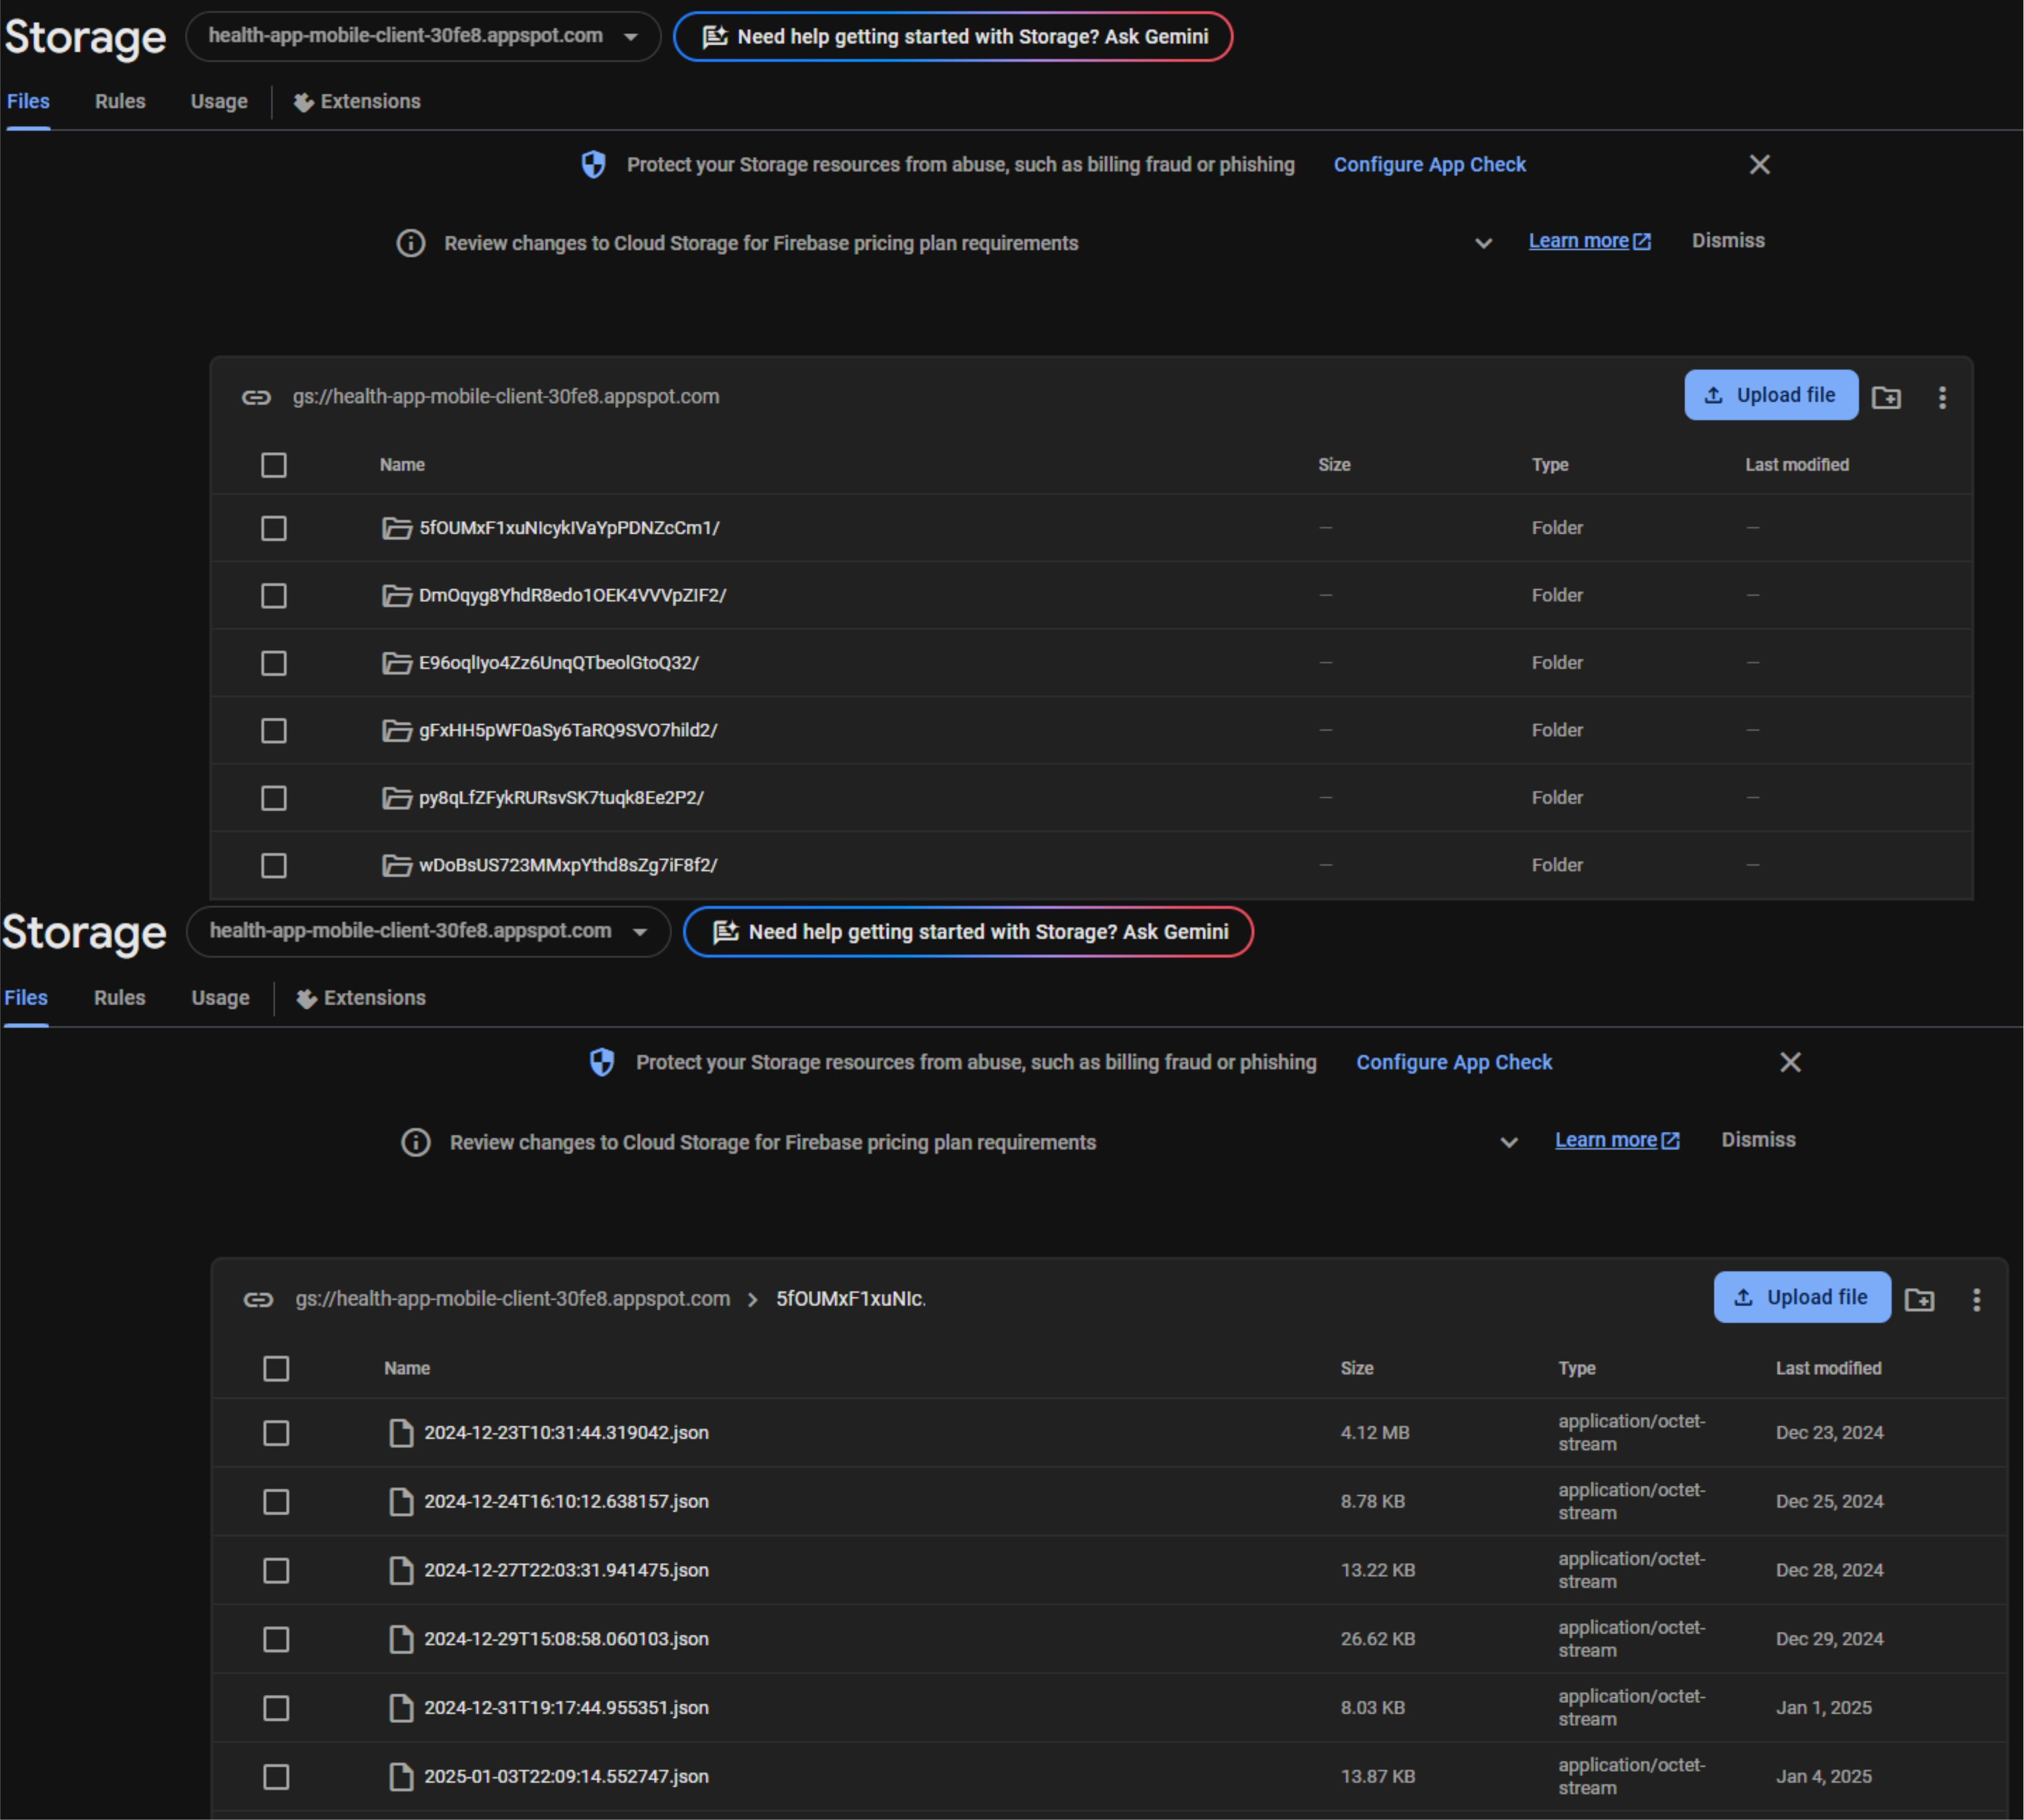
\includegraphics[width=1.0\linewidth]{./images/backup.jpg}
    \caption{Cloud Storage view of the users folder, uniquely named with userIds(left) and view of a single user folder containing the JSON files of the backup, uniquely named with the timestamp (right).}
\end{figure*}

\begin{figure*}
    \centering
    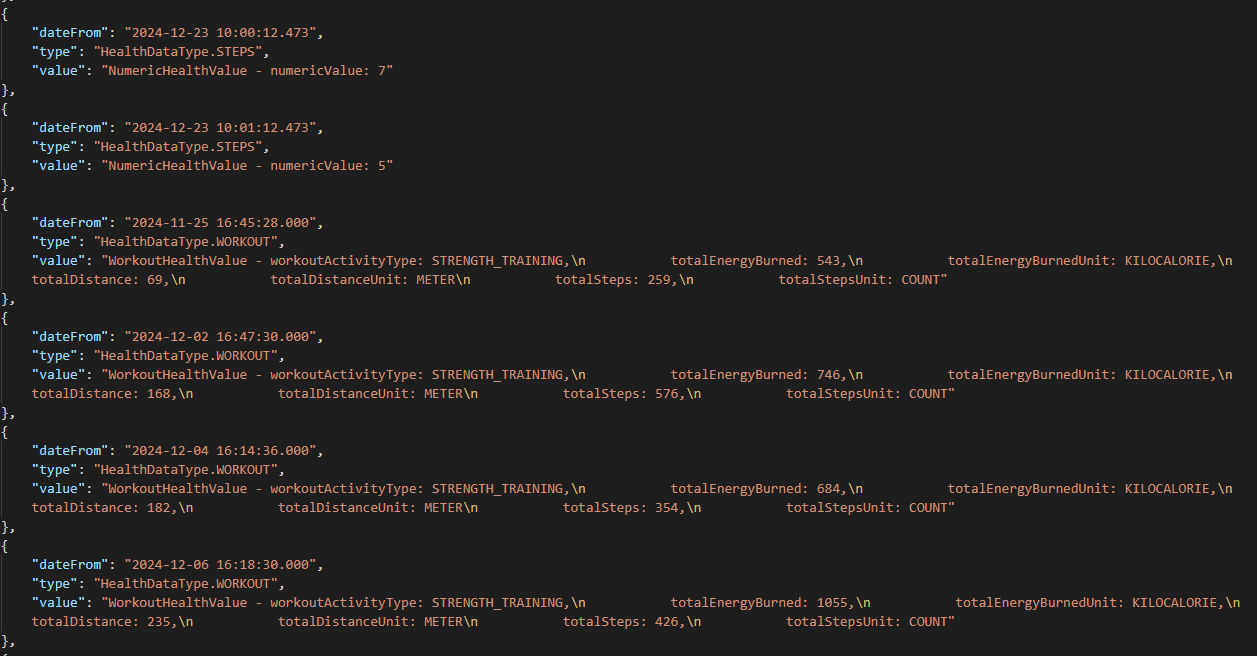
\includegraphics[width=1.0\linewidth]{./images/backup_json.png}
    \caption{Sample content of a json file of the backup, containing the health data of the user.}
\end{figure*}
\clearpage
\subsection{Notifications}
\label{subsec:notifications}
In order to satisfy the notifications requirements (see \cref{tab:fr3}), a notification system was designed and implemented. The notification system was designed with a cyclical behaviour. 
\newline The number of days that a full cycle of notification takes to go across all phases depends on the \texttt{assessment\_period} parameter inside the \texttt{notifications\_text} collection, editable by the admin. Infact, the scheduling of each notification during the different phases is not immediate but depends on the \texttt{assessment\_period} field and it is calculated based on that (\texttt{assessment\_period}/4 for each phase).  
\newline The main cycle is composed of four phases, with the \texttt{current\_notification} field initialized to the first phase, and employed to identify the current one. The phases are the following:
\begin{enumerate}[nosep] % 'nosep' removes extra spacing between items
    \item In the first phase, the first notification is sent and prompts the user to complete a test in order to assess his balance capabilities. In this case, the \texttt{current\_notification} field has as value body\_test\_balance.
    \item Once the user inserted his body balance data, the \texttt{current\_notification} field is updated to body\_test\_strength and the second phase begins. Another notification is sent, in this case to assess the physical strength of the user. 
    \item Once the user inserted his body strength data, the \texttt{current\_notification} field is updated to emotional\_life\_test and the third phase begins. Another notification is sent, in this case to assess the mood and emotional status of the user.
    \item Once the user inserted his emotional data, the \texttt{current\_notification} field is updated to assessment and the last phase begins. Another notification is sent, in this case opening an assessment based on the data provided by the user instead of prompting him to insert data, so that the user can see a period assessment each \texttt{assessment\_period} days. At this point the cycle restarts from the first phase.
\end{enumerate}

\noindent For all those phases there is of course the possibility to ignore the notification by discarding it. In this case to further prompt the user into an active participation, the same notification is rescheduled with an higher frequency. This howewer is performed for a limited amount of times. This is where the \texttt{notification\_counter} fields comes into: each time an user discard a notification is incremeted for a maximum of three times (from 0 to 2 included). When the counter reaches the maximum value, the notification is not rescheduled anymore and that specific phase is skipped, moving to the next one and resetting the counter to 0.
\newpage \noindent A separate lifecycle is used to manage the food interaction instead: in this case the frequency is daily, and in case the user discards the notification is simply rescheduled again. 
\newline The \texttt{NotificationService} class was employed to handle this logic, with two main methods employed to handle the two separate lifecycles: \texttt{scheduleNotification} for the main cycle and \texttt{scheduleFoodNotification} for the food cycle. These methods are called ad each applicaiton startup to schedule the notification, handling the case where the notifications have already been scheduled. Before these two methods the \texttt{initializeNotification} method is called to initialize the notifications and setup the listeners to hadle notification creation, opening and discarding. To practically schedule the notifications and use the listeners the \texttt{awesome\_notifications} API have been employed. 

\begin{figure*}
    \centering
    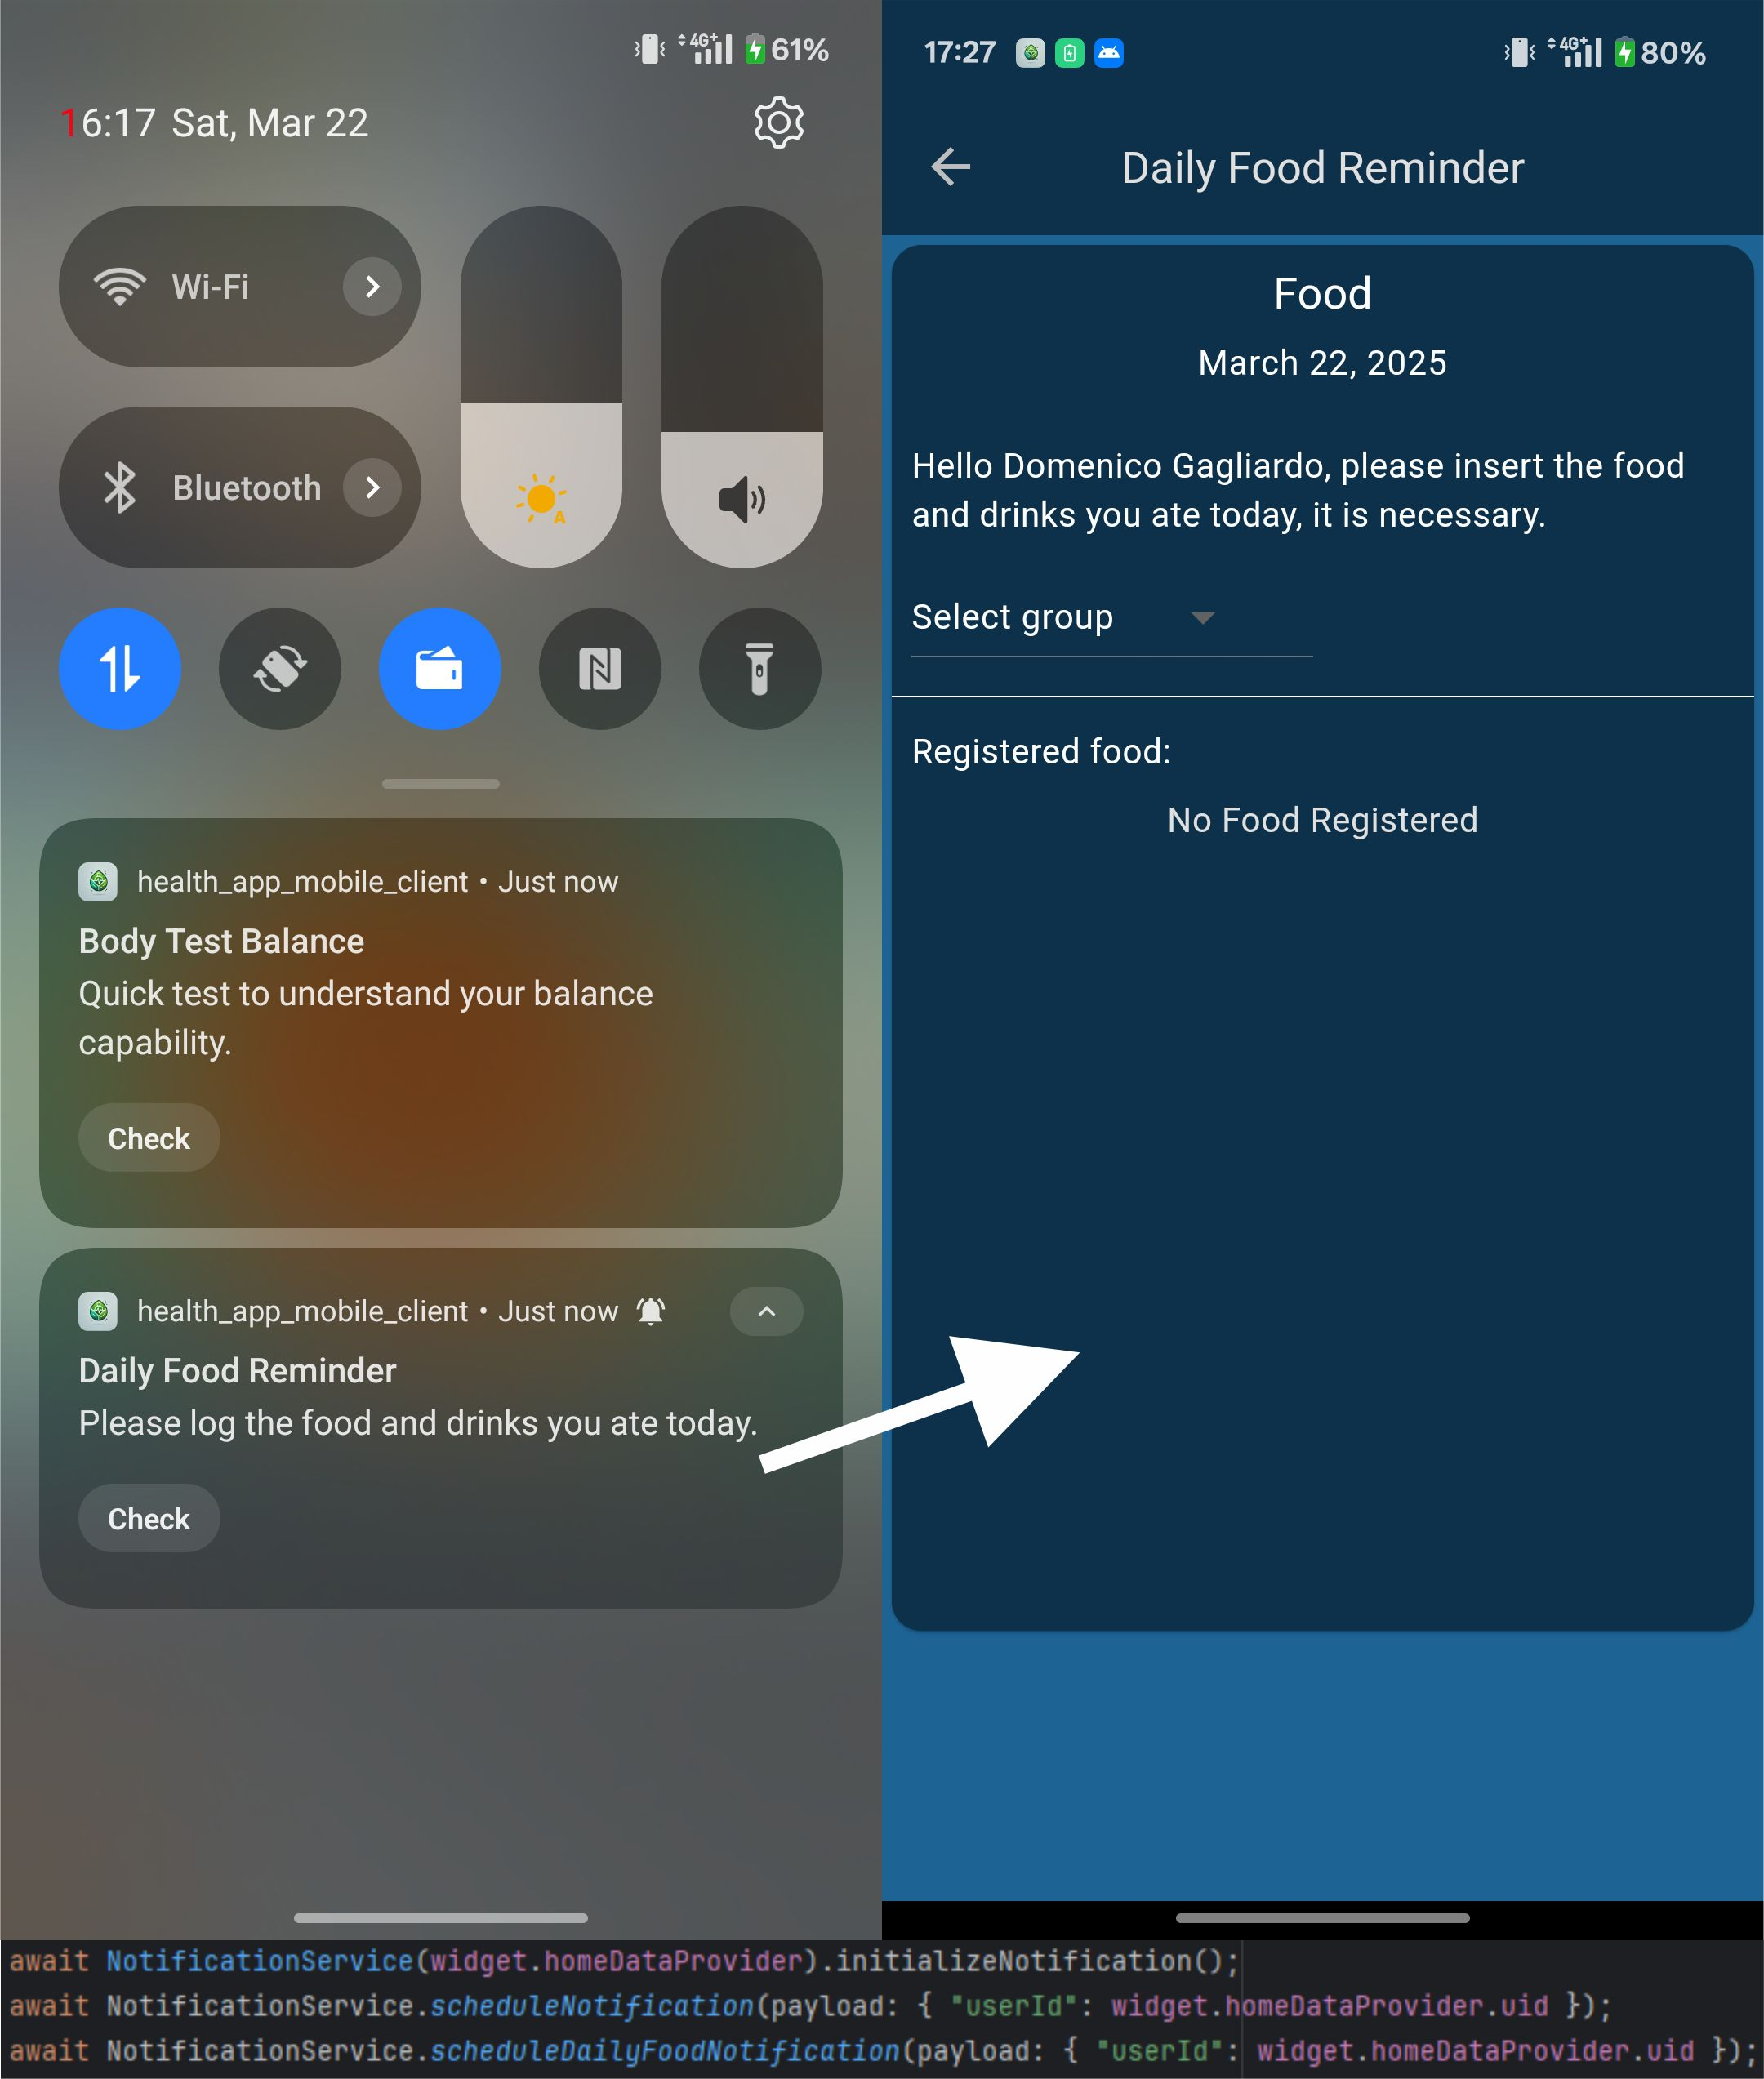
\includegraphics[width=0.7\linewidth]{./images/notifications.jpg}
    \caption{Example of the notifications sent (left), of the food form opened from the notification (right) and function call at application startup (bottom).}
\end{figure*}

\subsection{Application Parameters}
\label{subsec:applicationParameters}
The application parameters were employed to customize the app behaviour and the user experience. These parameters were used to perform the onBoarding, but also for the input forms (food form, body balance form, emotional forn and so on), present both in the graphs (giving the possibility to the user to enter data) and in the notifications, having used the same widgets in both cases.
\newline Coming to their usage, it is possible to make a practical distinction by using the \texttt{notifications\_text} collection documents to understand how they were used (see \cref{subsubsec:cloudFirestoreDatabase}):
\begin{itemize}[nosep] % 'nosep' removes extra spacing between items
    \item Firstly the \texttt{parameters} document and the user metrics were considered: the \newline\texttt{assessment\_period} and \texttt{coach\_name} parameters were firstly fetched, together with the user wearable device (\texttt{wearable} field, available for each user inside the \texttt{users} collection \texttt{metrics} field, among user personal information) and the username, directly fetched from the authentication session inside the application.
    \item Then, considering the other two documents of the \texttt{notifications\_text}, one of the two was fetched, depending on the language. At this point, since each string field contains placeholders for the parameter mentioned before, a pre-processing step was performed to replace those placeholders with the actual values, in order to obtain fields customized with the admin parameters (coach\_name and assessment\_period) but also user-tailored with the specific username and wearable device. 
\end{itemize}

\noindent The whole parameter logic is based upon the \texttt{fetchNotificationsText} function. Here the user language is fetched. Then the four parameters, initialized with default values, are fetched and then overriden when the \texttt{fetchParameters} function is called. After that, the \texttt{fetchNotificationsText} retrieves the \texttt{notifications\_text} parameters based on the language and the \texttt{replacePlaceholders} function is executed for each string field to replace the fields correctly. All those function are defined and present in the \texttt{HomeDataProvider} class in order to be easily accessible in the whole application, wherever these parameters are needed.

\begin{figure*}
    \centering
    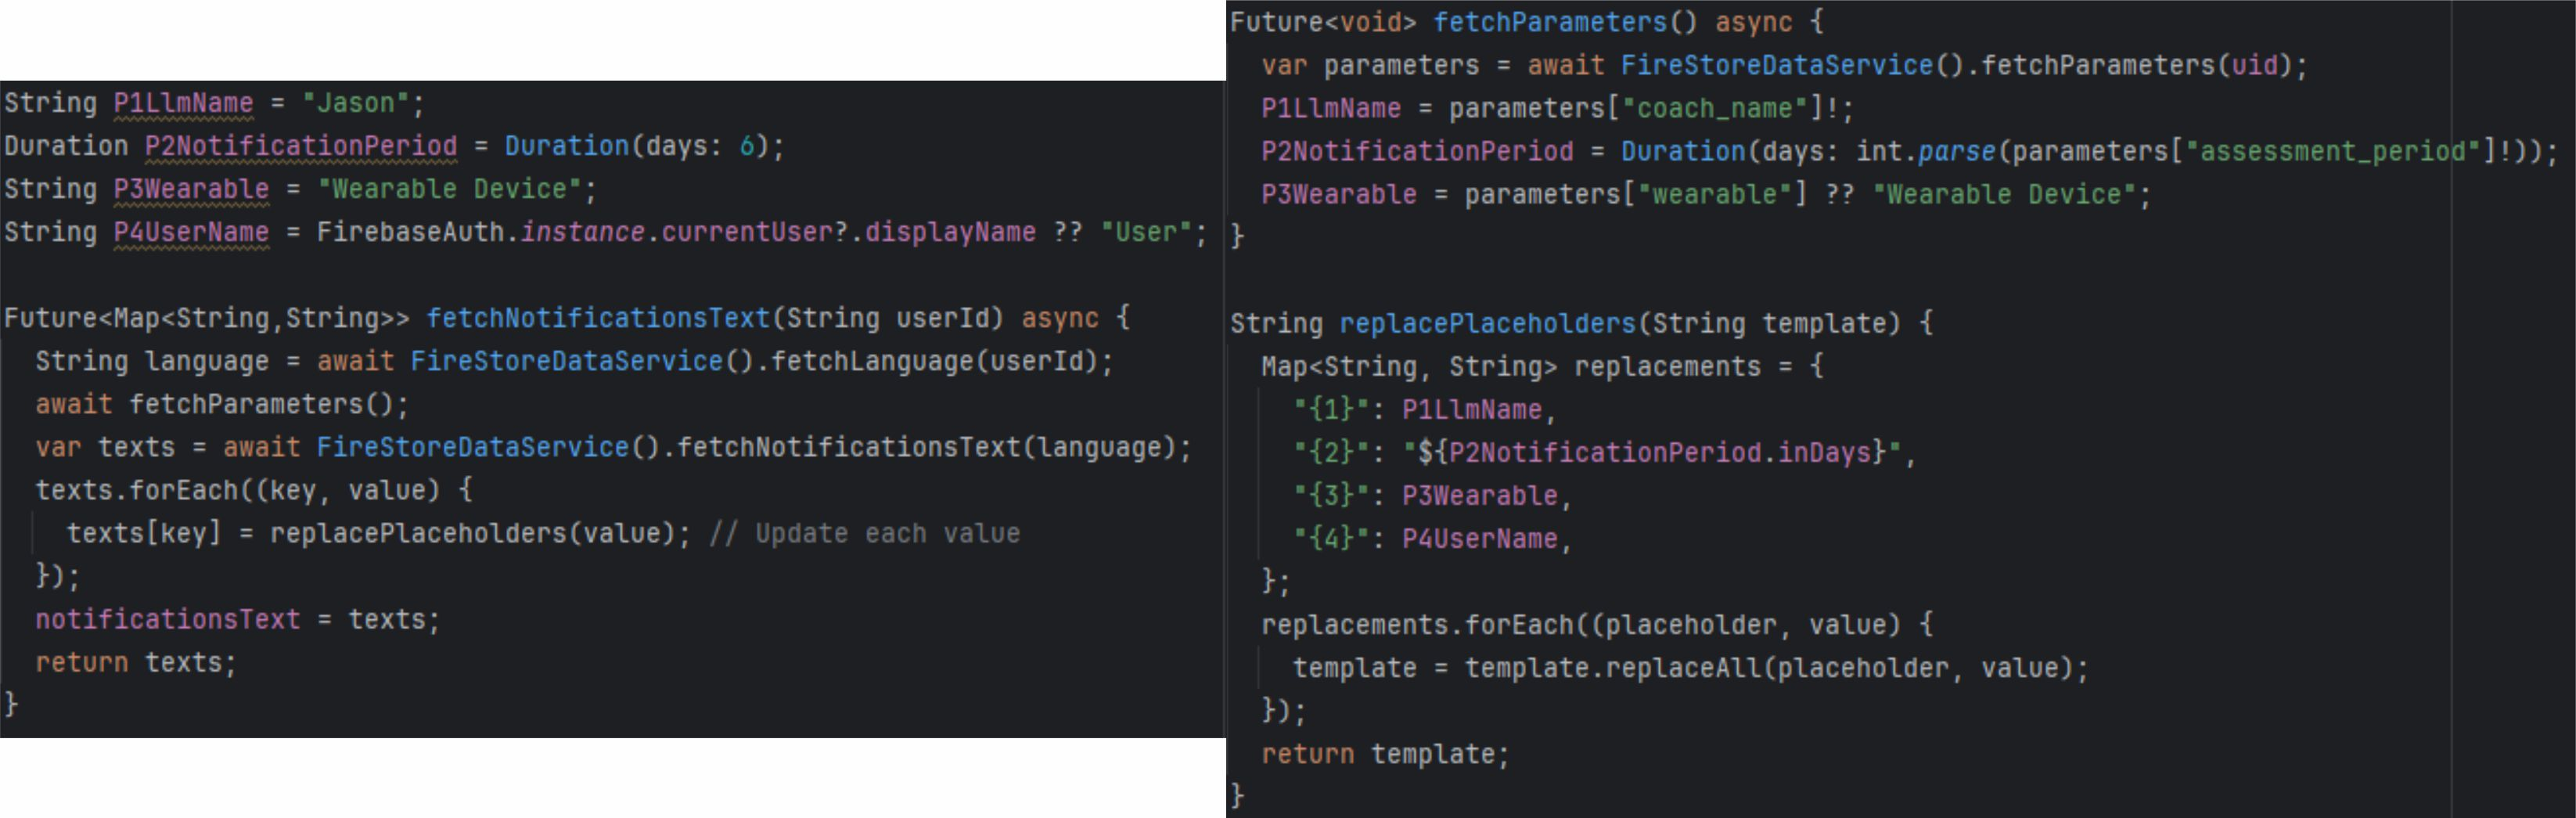
\includegraphics[width=1.0\linewidth]{./images/parameters.jpg}
    \caption{Parameter fetch flow.}
\end{figure*}

\subsection{Web Application}
To cover the admin requirements (see \cref{tab:fr2}) and allow the edit of the application parameters and the lessons/quizzes management, a react web application was employed.
\newline The application leverages on the firebase dependency \cite{Firebase} to enforce both authentication (see \cref{subsubsec:firebaseAuthentication}) and parameters editing.
\newline The application easily allows the admin to find which parameter to edit through a sidebar, that highlights the different parameters so that the admin can easily find which parameter wants to edit. The application also allows to change the language of the app through a dropdown, so that the admin can see the italian version of the parameters when it is needed, to edit them accordingly. In that case, speaking of parameters, only editing is possible and no deletion can be performed through the application.   
\newline Considering lesson and quiz management instead, there is the possibility to add, edit and delete lessons and quizzes. The addition and deletion operations have been done atomically in a transaction, in order to add lesson and quiz together, as well as deleting them together. This in order to link the lesson with the quiz through the \texttt{quizId} field and avoid inconsistencies like a quiz with no lesson or viceversa, which would have required at least a dedicated screen to let the admin link them together. Additional sections have been added to the sidebar to allow to perform these operations. In particular there are the \texttt{Add Lesson/Quiz} section, to add a lesson with the corresponding quiz. Then the \texttt{Lessons} section to view, edit and delete the lessons along with the quizzes, and the \texttt{Quizzes} section to view and edit the quizzes. 
\newpage \noindent The edit operations were performed with the \texttt{updateDoc} method, that allows to update in the document only the fields provided, while the add and delete operations were performed transactionally, respectively with \texttt{transaction.set}  and \texttt{transaction.delete} methods.

\begin{figure*}
    \centering
    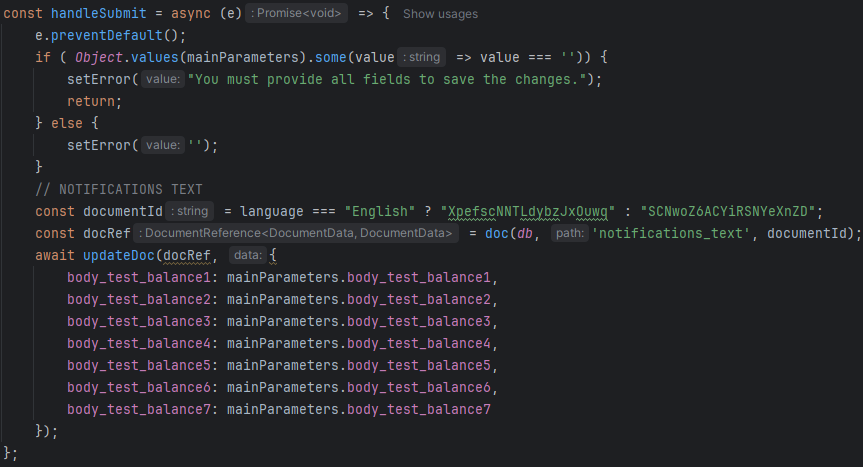
\includegraphics[width=1.0\linewidth]{./images/bodyTestBalanceParameters.png}
    \caption{Example usage of parameters update (body\_test\_balance).}
\end{figure*}

\begin{figure*}
    \centering
    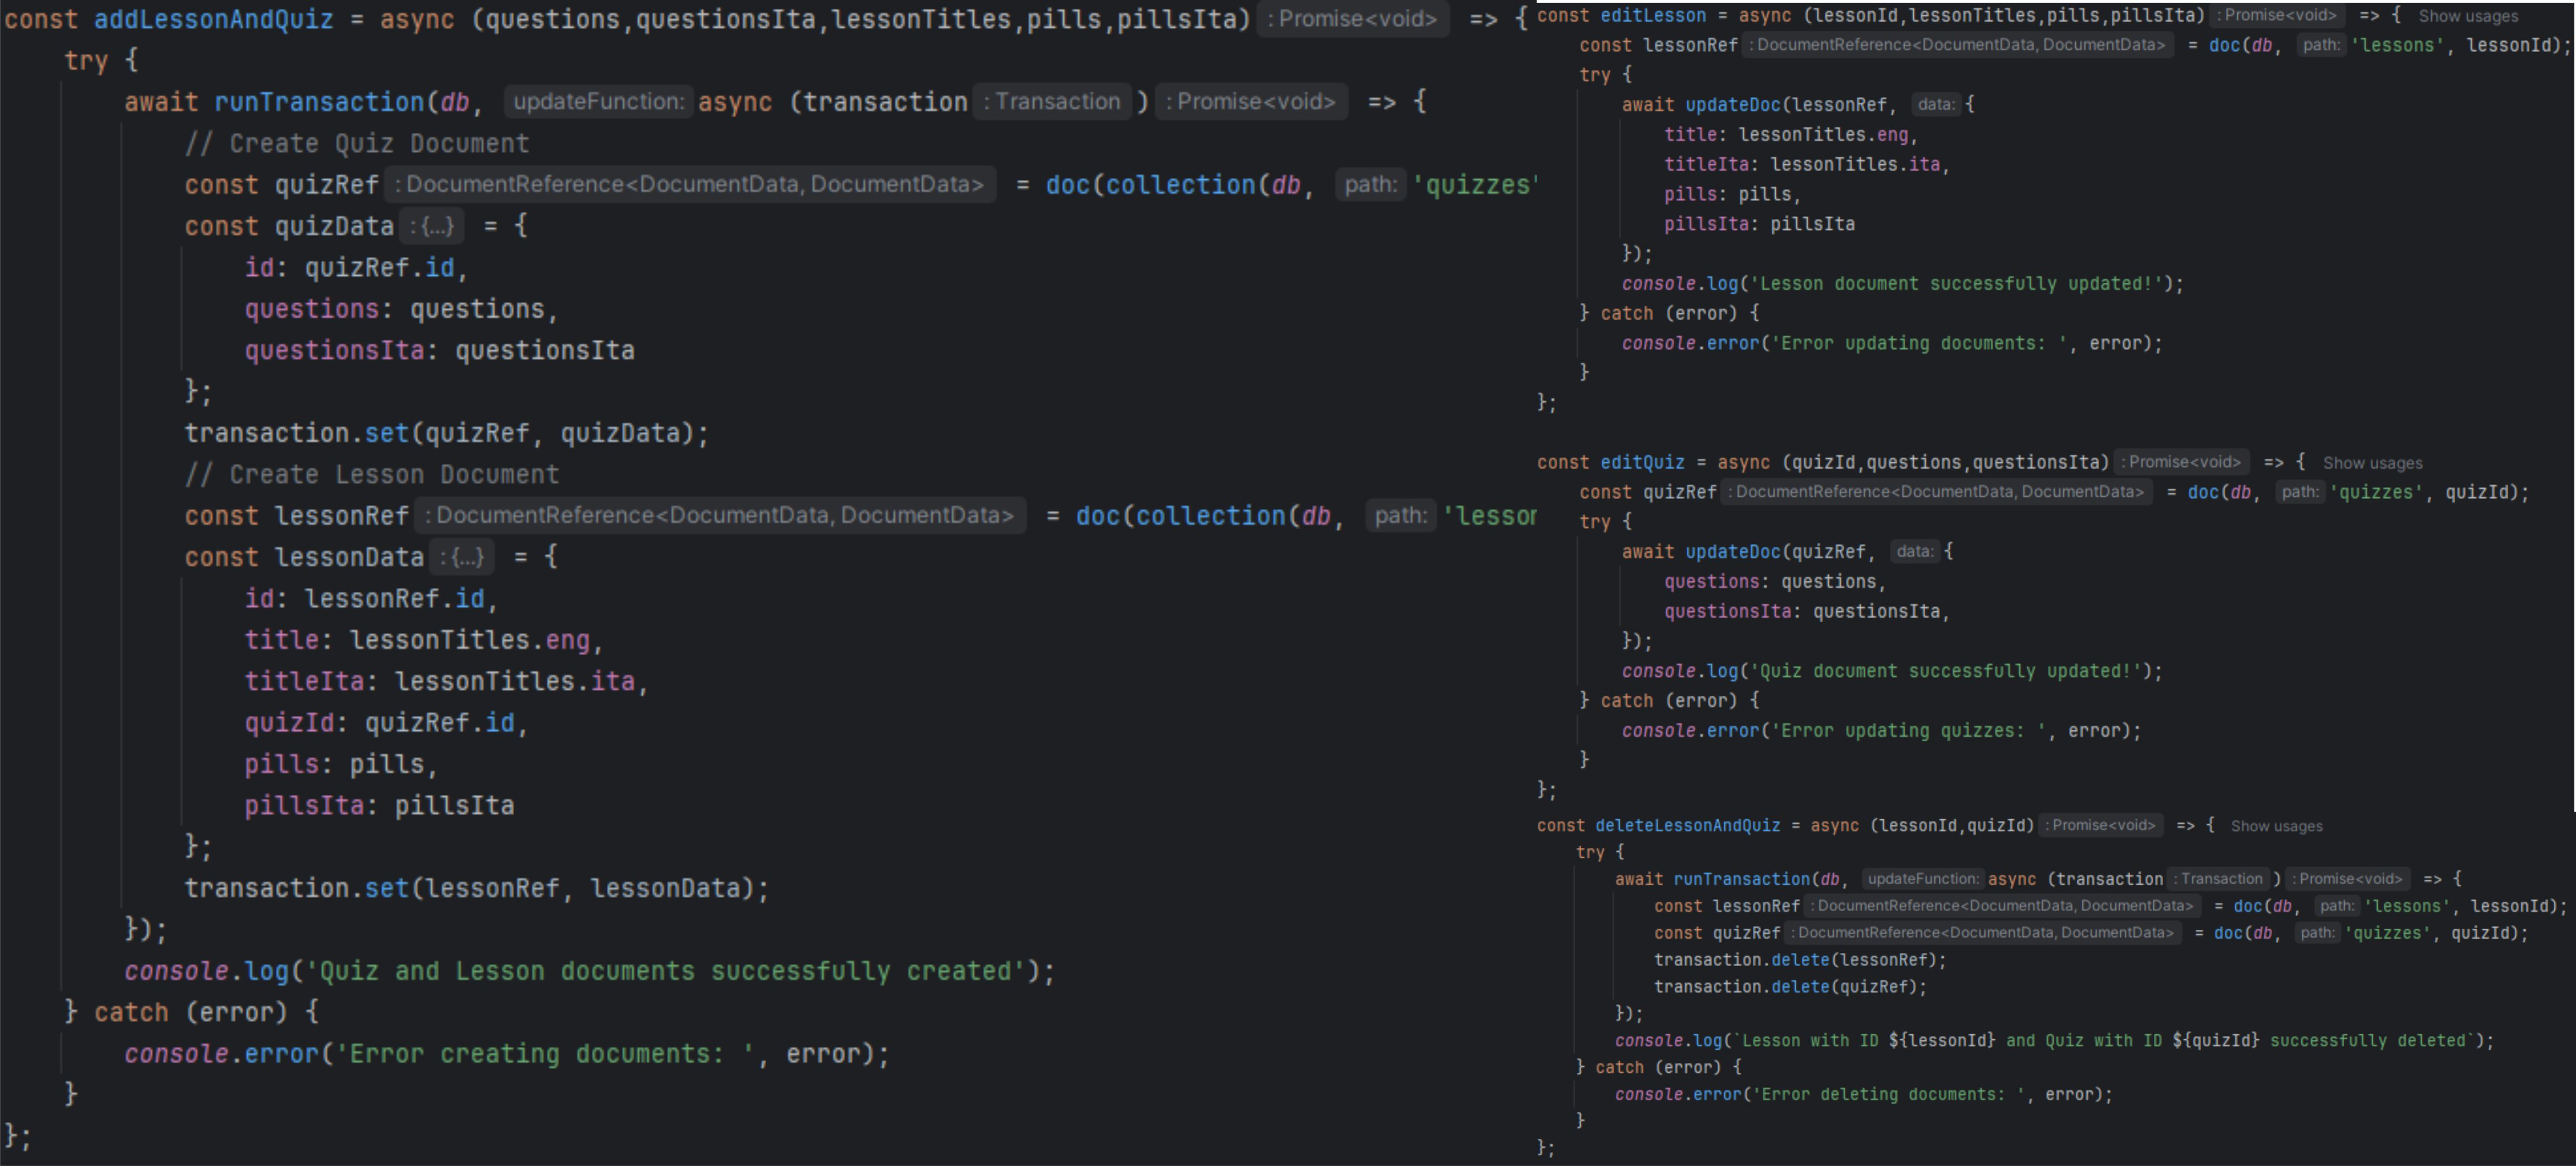
\includegraphics[width=1.0\linewidth]{./images/lessonsQuizzesParameters.jpg}
    \caption{Lessons And Quizzes database operations.}
\end{figure*}
